
    \documentclass{beamer}
    \usepackage{graphicx}
    \usepackage{Sweave}
    \usepackage{multicol}
    \usepackage{tikz}
    \usepackage{caption}    \setbeamertemplate{caption}{\raggedright\insertcaption\par}
    \usepackage[font={small}]{caption}
    \usetheme{Madrid}
    \usecolortheme{default}
    \setbeamertemplate{caption}[default]
    \makeatletter
    \setbeamertemplate{frametitle}
    {
        \ifbeamercolorempty[bg]{frametitle}{}{\nointerlineskip}
        \@tempdima=\textwidth
        \advance\@tempdima by\beamer@leftmargin
        \advance\@tempdima by\beamer@rightmargin
        \vskip1ex
        \begin{beamercolorbox}[sep=8pt,center,colsep=-4bp,rounded=true]{frametitle}
            \usebeamerfont{frametitle}
            \vbox{}\vskip-1ex
            \if@tempswa\else\csname beamer@ftecenter\endcsname\fi
            \strut\insertframetitle\strut\par
            {
                \ifx\insertframesubtitle\@empty
                \else
                {\usebeamerfont{framesubtitle}\usebeamercolor[fg]{framesubtitle}\insertframesubtitle\strut\par}%
                \fi
            }
            \vskip-1ex
            \if@tempswa\else\vskip-.3cm\fi
        \end{beamercolorbox}
    }
    \makeatother
    \setbeamertemplate{caption}{\raggedright\insertcaption\par}    \title{I love math but does she love me?}
    \subtitle{The analysis of PISA 2012 dataset.}
    \author[M. Futrega, \L. Rajkowski]{Micha\l\ Futrega and \L ukasz Rajkowski}
    \institute[MIM UW]{Faculty of Mathematics, University of Warsaw}
    \date{\today}    \setbeamertemplate{section in toc}{\inserttocsectionnumber.~\inserttocsection}
    \beamertemplatenavigationsymbolsempty
    
    \newcommand\AddButton{
    \setbeamertemplate{background canvas}{
    \begin{tikzpicture}[remember picture,overlay]
    \node[anchor=west] at ([yshift=20pt,xshift=1em]current page.south west)
      {\hyperlink{toc}{\beamergotobutton{Table of contests}}};
    \end{tikzpicture}
      }
    }    \begin{document}
    \begin{frame}
        \titlepage
        \center{\footnotesize We observed that countries where the affection to mathematics 
goes hand in hand with test results is ranked higher than country where there is no such correlation. 
}
    \end{frame}    \begin{frame}[label=toc] 
    \frametitle{List of countries} 
    \begin{multicols}{4}
    \scriptsize
    \tableofcontents
    \end{multicols}
    \end{frame}
\Sconcordance{concordance:report.tex:report.Rnw:%
24 1 20 4 0 1 1 28 0 1 1 3 0 1 1 9 0 1 1 5 0 1 1 5 0 1 2 1 1 1 59 324 0 %
1 2 1 1}

\AddButton\section{ Albania }\begin{frame}[t, fragile=singleslide]\frametitle{ Albania }\vspace*{-.4cm}\begin{figure}\begin{minipage}[t]{.52\textwidth}\centering\includegraphics[width=3.2cm, angle=270]{plots/temp1_Albania.eps}\caption*{\scriptsize 
        {\bf Boxplots} of the test score.
        The number on the box is the percentage of students within the group.
        It is also indicated by the fill.}\vspace{-.4cm}\fontsize{ 5 }{ 6 } \verb|aread("LRajkowski/pisa/b22043c6b905a5c90cd4e423bdcf4c11")|\end{minipage}\begin{minipage}[t]{.44\textwidth}\centering\includegraphics[width=3.2cm, angle=270]{plots/temp2_Albania.eps}\caption*{\scriptsize 
        {\bf Density estimation} of the test score within the groups of 
        {\color{red} (strong) likers} and {\color{blue}(strong) dislikers}.}\vspace{-.4cm}\fontsize{ 5 }{ 6 } \verb|aread("LRajkowski/pisa/12b45a31bcd8816e9ef96a91c82bcf4c")|\end{minipage}\\\vspace{-2.5cm}\end{figure}\begin{figure}\centering \includegraphics[width=6.0cm, height=10.0cm, angle=270]{plots/temp3_Albania.eps}\vspace{-2.5cm}\caption*{\scriptsize Albania  mean score is \ {\Large\bf\color{red} 58 } out of  65  countries}\vspace*{-.4cm}\fontsize{ 5 }{ 6 } \verb|aread("LRajkowski/pisa/9b2abf709f330722d9cf30adfa4f0da1")|\end{figure}\end{frame}\AddButton\section{ Argentina }\begin{frame}[t, fragile=singleslide]\frametitle{ Argentina }\vspace*{-.4cm}\begin{figure}\begin{minipage}[t]{.52\textwidth}\centering\includegraphics[width=3.2cm, angle=270]{plots/temp1_Argentina.eps}\caption*{\scriptsize 
        {\bf Boxplots} of the test score.
        The number on the box is the percentage of students within the group.
        It is also indicated by the fill.}\vspace{-.4cm}\fontsize{ 5 }{ 6 } \verb|aread("LRajkowski/pisa/2abba7d8c78e47fb0382709dc17ece2b")|\end{minipage}\begin{minipage}[t]{.44\textwidth}\centering\includegraphics[width=3.2cm, angle=270]{plots/temp2_Argentina.eps}\caption*{\scriptsize 
        {\bf Density estimation} of the test score within the groups of 
        {\color{red} (strong) likers} and {\color{blue}(strong) dislikers}.}\vspace{-.4cm}\fontsize{ 5 }{ 6 } \verb|aread("LRajkowski/pisa/e7fee9010db7f0949ba7cca3418e238d")|\end{minipage}\\\vspace{-2.5cm}\end{figure}\begin{figure}\centering \includegraphics[width=6.0cm, height=10.0cm, angle=270]{plots/temp3_Argentina.eps}\vspace{-2.5cm}\caption*{\scriptsize Argentina  mean score is \ {\Large\bf\color{red} 57 } out of  65  countries}\vspace*{-.4cm}\fontsize{ 5 }{ 6 } \verb|aread("LRajkowski/pisa/9134e20d2ffe983c5323138e7992b091")|\end{figure}\end{frame}\AddButton\section{ Australia }\begin{frame}[t, fragile=singleslide]\frametitle{ Australia }\vspace*{-.4cm}\begin{figure}\begin{minipage}[t]{.52\textwidth}\centering\includegraphics[width=3.2cm, angle=270]{plots/temp1_Australia.eps}\caption*{\scriptsize 
        {\bf Boxplots} of the test score.
        The number on the box is the percentage of students within the group.
        It is also indicated by the fill.}\vspace{-.4cm}\fontsize{ 5 }{ 6 } \verb|aread("LRajkowski/pisa/3b169564db2606226357a922a89d3097")|\end{minipage}\begin{minipage}[t]{.44\textwidth}\centering\includegraphics[width=3.2cm, angle=270]{plots/temp2_Australia.eps}\caption*{\scriptsize 
        {\bf Density estimation} of the test score within the groups of 
        {\color{red} (strong) likers} and {\color{blue}(strong) dislikers}.}\vspace{-.4cm}\fontsize{ 5 }{ 6 } \verb|aread("LRajkowski/pisa/e626167841e44be4f6a5290fabb23a50")|\end{minipage}\\\vspace{-2.5cm}\end{figure}\begin{figure}\centering \includegraphics[width=6.0cm, height=10.0cm, angle=270]{plots/temp3_Australia.eps}\vspace{-2.5cm}\caption*{\scriptsize Australia  mean score is \ {\Large\bf\color{red} 26 } out of  65  countries}\vspace*{-.4cm}\fontsize{ 5 }{ 6 } \verb|aread("LRajkowski/pisa/e21731ab17f8e53645a2beca76151a8a")|\end{figure}\end{frame}\AddButton\section{ Austria }\begin{frame}[t, fragile=singleslide]\frametitle{ Austria }\vspace*{-.4cm}\begin{figure}\begin{minipage}[t]{.52\textwidth}\centering\includegraphics[width=3.2cm, angle=270]{plots/temp1_Austria.eps}\caption*{\scriptsize 
        {\bf Boxplots} of the test score.
        The number on the box is the percentage of students within the group.
        It is also indicated by the fill.}\vspace{-.4cm}\fontsize{ 5 }{ 6 } \verb|aread("LRajkowski/pisa/1cf13a29ffbca2ef64e5005199b9dee9")|\end{minipage}\begin{minipage}[t]{.44\textwidth}\centering\includegraphics[width=3.2cm, angle=270]{plots/temp2_Austria.eps}\caption*{\scriptsize 
        {\bf Density estimation} of the test score within the groups of 
        {\color{red} (strong) likers} and {\color{blue}(strong) dislikers}.}\vspace{-.4cm}\fontsize{ 5 }{ 6 } \verb|aread("LRajkowski/pisa/b1edc2ef8a0bfa1c81f51accdd73cf69")|\end{minipage}\\\vspace{-2.5cm}\end{figure}\begin{figure}\centering \includegraphics[width=6.0cm, height=10.0cm, angle=270]{plots/temp3_Austria.eps}\vspace{-2.5cm}\caption*{\scriptsize Austria  mean score is \ {\Large\bf\color{red} 18 } out of  65  countries}\vspace*{-.4cm}\fontsize{ 5 }{ 6 } \verb|aread("LRajkowski/pisa/f6a58903ef86da0c8bbde00dadfa40e8")|\end{figure}\end{frame}\AddButton\section{ Belgium }\begin{frame}[t, fragile=singleslide]\frametitle{ Belgium }\vspace*{-.4cm}\begin{figure}\begin{minipage}[t]{.52\textwidth}\centering\includegraphics[width=3.2cm, angle=270]{plots/temp1_Belgium.eps}\caption*{\scriptsize 
        {\bf Boxplots} of the test score.
        The number on the box is the percentage of students within the group.
        It is also indicated by the fill.}\vspace{-.4cm}\fontsize{ 5 }{ 6 } \verb|aread("LRajkowski/pisa/07632400f5dcef989a0492d90be0d196")|\end{minipage}\begin{minipage}[t]{.44\textwidth}\centering\includegraphics[width=3.2cm, angle=270]{plots/temp2_Belgium.eps}\caption*{\scriptsize 
        {\bf Density estimation} of the test score within the groups of 
        {\color{red} (strong) likers} and {\color{blue}(strong) dislikers}.}\vspace{-.4cm}\fontsize{ 5 }{ 6 } \verb|aread("LRajkowski/pisa/a79db3700a2221b17564ccfce732940a")|\end{minipage}\\\vspace{-2.5cm}\end{figure}\begin{figure}\centering \includegraphics[width=6.0cm, height=10.0cm, angle=270]{plots/temp3_Belgium.eps}\vspace{-2.5cm}\caption*{\scriptsize Belgium  mean score is \ {\Large\bf\color{red} 12 } out of  65  countries}\vspace*{-.4cm}\fontsize{ 5 }{ 6 } \verb|aread("LRajkowski/pisa/6a199e925e1a43c075ee799090b57d8e")|\end{figure}\end{frame}\AddButton\section{ Brazil }\begin{frame}[t, fragile=singleslide]\frametitle{ Brazil }\vspace*{-.4cm}\begin{figure}\begin{minipage}[t]{.52\textwidth}\centering\includegraphics[width=3.2cm, angle=270]{plots/temp1_Brazil.eps}\caption*{\scriptsize 
        {\bf Boxplots} of the test score.
        The number on the box is the percentage of students within the group.
        It is also indicated by the fill.}\vspace{-.4cm}\fontsize{ 5 }{ 6 } \verb|aread("LRajkowski/pisa/06fbe994b1b39829caaeb97389306376")|\end{minipage}\begin{minipage}[t]{.44\textwidth}\centering\includegraphics[width=3.2cm, angle=270]{plots/temp2_Brazil.eps}\caption*{\scriptsize 
        {\bf Density estimation} of the test score within the groups of 
        {\color{red} (strong) likers} and {\color{blue}(strong) dislikers}.}\vspace{-.4cm}\fontsize{ 5 }{ 6 } \verb|aread("LRajkowski/pisa/448f58d7242b3b2d6283bcc97ee90004")|\end{minipage}\\\vspace{-2.5cm}\end{figure}\begin{figure}\centering \includegraphics[width=6.0cm, height=10.0cm, angle=270]{plots/temp3_Brazil.eps}\vspace{-2.5cm}\caption*{\scriptsize Brazil  mean score is \ {\Large\bf\color{red} 62 } out of  65  countries}\vspace*{-.4cm}\fontsize{ 5 }{ 6 } \verb|aread("LRajkowski/pisa/d9253ddb47ab550f0e7b24823a77624d")|\end{figure}\end{frame}\AddButton\section{ Bulgaria }\begin{frame}[t, fragile=singleslide]\frametitle{ Bulgaria }\vspace*{-.4cm}\begin{figure}\begin{minipage}[t]{.52\textwidth}\centering\includegraphics[width=3.2cm, angle=270]{plots/temp1_Bulgaria.eps}\caption*{\scriptsize 
        {\bf Boxplots} of the test score.
        The number on the box is the percentage of students within the group.
        It is also indicated by the fill.}\vspace{-.4cm}\fontsize{ 5 }{ 6 } \verb|aread("LRajkowski/pisa/33d683b74a7e43321ab602f5c552e00a")|\end{minipage}\begin{minipage}[t]{.44\textwidth}\centering\includegraphics[width=3.2cm, angle=270]{plots/temp2_Bulgaria.eps}\caption*{\scriptsize 
        {\bf Density estimation} of the test score within the groups of 
        {\color{red} (strong) likers} and {\color{blue}(strong) dislikers}.}\vspace{-.4cm}\fontsize{ 5 }{ 6 } \verb|aread("LRajkowski/pisa/6925dc48d6938c4e18de333fb2c5b10b")|\end{minipage}\\\vspace{-2.5cm}\end{figure}\begin{figure}\centering \includegraphics[width=6.0cm, height=10.0cm, angle=270]{plots/temp3_Bulgaria.eps}\vspace{-2.5cm}\caption*{\scriptsize Bulgaria  mean score is \ {\Large\bf\color{red} 48 } out of  65  countries}\vspace*{-.4cm}\fontsize{ 5 }{ 6 } \verb|aread("LRajkowski/pisa/851dc803700a5ad7d0a88957dce56fca")|\end{figure}\end{frame}\AddButton\section{ Canada }\begin{frame}[t, fragile=singleslide]\frametitle{ Canada }\vspace*{-.4cm}\begin{figure}\begin{minipage}[t]{.52\textwidth}\centering\includegraphics[width=3.2cm, angle=270]{plots/temp1_Canada.eps}\caption*{\scriptsize 
        {\bf Boxplots} of the test score.
        The number on the box is the percentage of students within the group.
        It is also indicated by the fill.}\vspace{-.4cm}\fontsize{ 5 }{ 6 } \verb|aread("LRajkowski/pisa/0116fddf448fa3604364ce080fd37e7a")|\end{minipage}\begin{minipage}[t]{.44\textwidth}\centering\includegraphics[width=3.2cm, angle=270]{plots/temp2_Canada.eps}\caption*{\scriptsize 
        {\bf Density estimation} of the test score within the groups of 
        {\color{red} (strong) likers} and {\color{blue}(strong) dislikers}.}\vspace{-.4cm}\fontsize{ 5 }{ 6 } \verb|aread("LRajkowski/pisa/4bf4e055fb1858d2a556feee84fec4ea")|\end{minipage}\\\vspace{-2.5cm}\end{figure}\begin{figure}\centering \includegraphics[width=6.0cm, height=10.0cm, angle=270]{plots/temp3_Canada.eps}\vspace{-2.5cm}\caption*{\scriptsize Canada  mean score is \ {\Large\bf\color{red} 17 } out of  65  countries}\vspace*{-.4cm}\fontsize{ 5 }{ 6 } \verb|aread("LRajkowski/pisa/2573bf1cd544aaaa85b2f916f66fa4de")|\end{figure}\end{frame}\AddButton\section{ Chile }\begin{frame}[t, fragile=singleslide]\frametitle{ Chile }\vspace*{-.4cm}\begin{figure}\begin{minipage}[t]{.52\textwidth}\centering\includegraphics[width=3.2cm, angle=270]{plots/temp1_Chile.eps}\caption*{\scriptsize 
        {\bf Boxplots} of the test score.
        The number on the box is the percentage of students within the group.
        It is also indicated by the fill.}\vspace{-.4cm}\fontsize{ 5 }{ 6 } \verb|aread("LRajkowski/pisa/a6680b175b35bd853739266886989cb2")|\end{minipage}\begin{minipage}[t]{.44\textwidth}\centering\includegraphics[width=3.2cm, angle=270]{plots/temp2_Chile.eps}\caption*{\scriptsize 
        {\bf Density estimation} of the test score within the groups of 
        {\color{red} (strong) likers} and {\color{blue}(strong) dislikers}.}\vspace{-.4cm}\fontsize{ 5 }{ 6 } \verb|aread("LRajkowski/pisa/b8ba3c320d0dd2bbc42bfbeec22f10ef")|\end{minipage}\\\vspace{-2.5cm}\end{figure}\begin{figure}\centering \includegraphics[width=6.0cm, height=10.0cm, angle=270]{plots/temp3_Chile.eps}\vspace{-2.5cm}\caption*{\scriptsize Chile  mean score is \ {\Large\bf\color{red} 47 } out of  65  countries}\vspace*{-.4cm}\fontsize{ 5 }{ 6 } \verb|aread("LRajkowski/pisa/32cc197b7647c336e7f18012a9c97ea8")|\end{figure}\end{frame}\AddButton\section{ China-Shanghai }\begin{frame}[t, fragile=singleslide]\frametitle{ China-Shanghai }\vspace*{-.4cm}\begin{figure}\begin{minipage}[t]{.52\textwidth}\centering\includegraphics[width=3.2cm, angle=270]{plots/temp1_China-Shanghai.eps}\caption*{\scriptsize 
        {\bf Boxplots} of the test score.
        The number on the box is the percentage of students within the group.
        It is also indicated by the fill.}\vspace{-.4cm}\fontsize{ 5 }{ 6 } \verb|aread("LRajkowski/pisa/d7382c416028fe5acd33096bfe4479b8")|\end{minipage}\begin{minipage}[t]{.44\textwidth}\centering\includegraphics[width=3.2cm, angle=270]{plots/temp2_China-Shanghai.eps}\caption*{\scriptsize 
        {\bf Density estimation} of the test score within the groups of 
        {\color{red} (strong) likers} and {\color{blue}(strong) dislikers}.}\vspace{-.4cm}\fontsize{ 5 }{ 6 } \verb|aread("LRajkowski/pisa/3f489127d3f9191d132a0713f719b590")|\end{minipage}\\\vspace{-2.5cm}\end{figure}\begin{figure}\centering \includegraphics[width=6.0cm, height=10.0cm, angle=270]{plots/temp3_China-Shanghai.eps}\vspace{-2.5cm}\caption*{\scriptsize China-Shanghai  mean score is \ {\Large\bf\color{red} 1 } out of  65  countries}\vspace*{-.4cm}\fontsize{ 5 }{ 6 } \verb|aread("LRajkowski/pisa/6473b8b25ac9067b575238daf8cbf5a6")|\end{figure}\end{frame}\AddButton\section{ Chinese Taipei }\begin{frame}[t, fragile=singleslide]\frametitle{ Chinese Taipei }\vspace*{-.4cm}\begin{figure}\begin{minipage}[t]{.52\textwidth}\centering\includegraphics[width=3.2cm, angle=270]{plots/temp1_ChineseTaipei.eps}\caption*{\scriptsize 
        {\bf Boxplots} of the test score.
        The number on the box is the percentage of students within the group.
        It is also indicated by the fill.}\vspace{-.4cm}\fontsize{ 5 }{ 6 } \verb|aread("LRajkowski/pisa/7eae4f0f190de2e246a70554ce47666b")|\end{minipage}\begin{minipage}[t]{.44\textwidth}\centering\includegraphics[width=3.2cm, angle=270]{plots/temp2_ChineseTaipei.eps}\caption*{\scriptsize 
        {\bf Density estimation} of the test score within the groups of 
        {\color{red} (strong) likers} and {\color{blue}(strong) dislikers}.}\vspace{-.4cm}\fontsize{ 5 }{ 6 } \verb|aread("LRajkowski/pisa/cab8483629d7f29c2871514d3132fcc2")|\end{minipage}\\\vspace{-2.5cm}\end{figure}\begin{figure}\centering \includegraphics[width=6.0cm, height=10.0cm, angle=270]{plots/temp3_ChineseTaipei.eps}\vspace{-2.5cm}\caption*{\scriptsize Chinese Taipei  mean score is \ {\Large\bf\color{red} 4 } out of  65  countries}\vspace*{-.4cm}\fontsize{ 5 }{ 6 } \verb|aread("LRajkowski/pisa/7e8ab4545aa40738fb578b62f3f94424")|\end{figure}\end{frame}\AddButton\section{ Colombia }\begin{frame}[t, fragile=singleslide]\frametitle{ Colombia }\vspace*{-.4cm}\begin{figure}\begin{minipage}[t]{.52\textwidth}\centering\includegraphics[width=3.2cm, angle=270]{plots/temp1_Colombia.eps}\caption*{\scriptsize 
        {\bf Boxplots} of the test score.
        The number on the box is the percentage of students within the group.
        It is also indicated by the fill.}\vspace{-.4cm}\fontsize{ 5 }{ 6 } \verb|aread("LRajkowski/pisa/38e272fa12fce96f4acdc9a7f80ae2ab")|\end{minipage}\begin{minipage}[t]{.44\textwidth}\centering\includegraphics[width=3.2cm, angle=270]{plots/temp2_Colombia.eps}\caption*{\scriptsize 
        {\bf Density estimation} of the test score within the groups of 
        {\color{red} (strong) likers} and {\color{blue}(strong) dislikers}.}\vspace{-.4cm}\fontsize{ 5 }{ 6 } \verb|aread("LRajkowski/pisa/3e0d2df8e018916a0df75788b8f45807")|\end{minipage}\\\vspace{-2.5cm}\end{figure}\begin{figure}\centering \includegraphics[width=6.0cm, height=10.0cm, angle=270]{plots/temp3_Colombia.eps}\vspace{-2.5cm}\caption*{\scriptsize Colombia  mean score is \ {\Large\bf\color{red} 60 } out of  65  countries}\vspace*{-.4cm}\fontsize{ 5 }{ 6 } \verb|aread("LRajkowski/pisa/0091a84f8fe07c7477d8fdc51796fbc3")|\end{figure}\end{frame}\AddButton\section{ Costa Rica }\begin{frame}[t, fragile=singleslide]\frametitle{ Costa Rica }\vspace*{-.4cm}\begin{figure}\begin{minipage}[t]{.52\textwidth}\centering\includegraphics[width=3.2cm, angle=270]{plots/temp1_CostaRica.eps}\caption*{\scriptsize 
        {\bf Boxplots} of the test score.
        The number on the box is the percentage of students within the group.
        It is also indicated by the fill.}\vspace{-.4cm}\fontsize{ 5 }{ 6 } \verb|aread("LRajkowski/pisa/a3b3344f1d02c7eb3b6bcc4d59f73eea")|\end{minipage}\begin{minipage}[t]{.44\textwidth}\centering\includegraphics[width=3.2cm, angle=270]{plots/temp2_CostaRica.eps}\caption*{\scriptsize 
        {\bf Density estimation} of the test score within the groups of 
        {\color{red} (strong) likers} and {\color{blue}(strong) dislikers}.}\vspace{-.4cm}\fontsize{ 5 }{ 6 } \verb|aread("LRajkowski/pisa/b197d549229a90f5d980d977d0a13204")|\end{minipage}\\\vspace{-2.5cm}\end{figure}\begin{figure}\centering \includegraphics[width=6.0cm, height=10.0cm, angle=270]{plots/temp3_CostaRica.eps}\vspace{-2.5cm}\caption*{\scriptsize Costa Rica  mean score is \ {\Large\bf\color{red} 56 } out of  65  countries}\vspace*{-.4cm}\fontsize{ 5 }{ 6 } \verb|aread("LRajkowski/pisa/3ae781b856cb6e4522a99ee89ea2b110")|\end{figure}\end{frame}\AddButton\section{ Croatia }\begin{frame}[t, fragile=singleslide]\frametitle{ Croatia }\vspace*{-.4cm}\begin{figure}\begin{minipage}[t]{.52\textwidth}\centering\includegraphics[width=3.2cm, angle=270]{plots/temp1_Croatia.eps}\caption*{\scriptsize 
        {\bf Boxplots} of the test score.
        The number on the box is the percentage of students within the group.
        It is also indicated by the fill.}\vspace{-.4cm}\fontsize{ 5 }{ 6 } \verb|aread("LRajkowski/pisa/3ed11151bc2223f743cba52a1252f22f")|\end{minipage}\begin{minipage}[t]{.44\textwidth}\centering\includegraphics[width=3.2cm, angle=270]{plots/temp2_Croatia.eps}\caption*{\scriptsize 
        {\bf Density estimation} of the test score within the groups of 
        {\color{red} (strong) likers} and {\color{blue}(strong) dislikers}.}\vspace{-.4cm}\fontsize{ 5 }{ 6 } \verb|aread("LRajkowski/pisa/7659f04ccb1cc8c66a88d00189da89ad")|\end{minipage}\\\vspace{-2.5cm}\end{figure}\begin{figure}\centering \includegraphics[width=6.0cm, height=10.0cm, angle=270]{plots/temp3_Croatia.eps}\vspace{-2.5cm}\caption*{\scriptsize Croatia  mean score is \ {\Large\bf\color{red} 41 } out of  65  countries}\vspace*{-.4cm}\fontsize{ 5 }{ 6 } \verb|aread("LRajkowski/pisa/9656a69c5fbe5960cbbb4744a68f68a9")|\end{figure}\end{frame}\AddButton\section{ Czech Republic }\begin{frame}[t, fragile=singleslide]\frametitle{ Czech Republic }\vspace*{-.4cm}\begin{figure}\begin{minipage}[t]{.52\textwidth}\centering\includegraphics[width=3.2cm, angle=270]{plots/temp1_CzechRepublic.eps}\caption*{\scriptsize 
        {\bf Boxplots} of the test score.
        The number on the box is the percentage of students within the group.
        It is also indicated by the fill.}\vspace{-.4cm}\fontsize{ 5 }{ 6 } \verb|aread("LRajkowski/pisa/c102a18cc76e8c799cd3779efb31594d")|\end{minipage}\begin{minipage}[t]{.44\textwidth}\centering\includegraphics[width=3.2cm, angle=270]{plots/temp2_CzechRepublic.eps}\caption*{\scriptsize 
        {\bf Density estimation} of the test score within the groups of 
        {\color{red} (strong) likers} and {\color{blue}(strong) dislikers}.}\vspace{-.4cm}\fontsize{ 5 }{ 6 } \verb|aread("LRajkowski/pisa/148c63979b3760afc123aee9f7390070")|\end{minipage}\\\vspace{-2.5cm}\end{figure}\begin{figure}\centering \includegraphics[width=6.0cm, height=10.0cm, angle=270]{plots/temp3_CzechRepublic.eps}\vspace{-2.5cm}\caption*{\scriptsize Czech Republic  mean score is \ {\Large\bf\color{red} 13 } out of  65  countries}\vspace*{-.4cm}\fontsize{ 5 }{ 6 } \verb|aread("LRajkowski/pisa/8c77949f442675f524077e6a18a06946")|\end{figure}\end{frame}\AddButton\section{ Denmark }\begin{frame}[t, fragile=singleslide]\frametitle{ Denmark }\vspace*{-.4cm}\begin{figure}\begin{minipage}[t]{.52\textwidth}\centering\includegraphics[width=3.2cm, angle=270]{plots/temp1_Denmark.eps}\caption*{\scriptsize 
        {\bf Boxplots} of the test score.
        The number on the box is the percentage of students within the group.
        It is also indicated by the fill.}\vspace{-.4cm}\fontsize{ 5 }{ 6 } \verb|aread("LRajkowski/pisa/7dabee387e63acfdd9e47d00046f4716")|\end{minipage}\begin{minipage}[t]{.44\textwidth}\centering\includegraphics[width=3.2cm, angle=270]{plots/temp2_Denmark.eps}\caption*{\scriptsize 
        {\bf Density estimation} of the test score within the groups of 
        {\color{red} (strong) likers} and {\color{blue}(strong) dislikers}.}\vspace{-.4cm}\fontsize{ 5 }{ 6 } \verb|aread("LRajkowski/pisa/8f61186df853500d45ca6062341de04a")|\end{minipage}\\\vspace{-2.5cm}\end{figure}\begin{figure}\centering \includegraphics[width=6.0cm, height=10.0cm, angle=270]{plots/temp3_Denmark.eps}\vspace{-2.5cm}\caption*{\scriptsize Denmark  mean score is \ {\Large\bf\color{red} 32 } out of  65  countries}\vspace*{-.4cm}\fontsize{ 5 }{ 6 } \verb|aread("LRajkowski/pisa/63ec260ebfc61c46305177309e8e8318")|\end{figure}\end{frame}\AddButton\section{ Estonia }\begin{frame}[t, fragile=singleslide]\frametitle{ Estonia }\vspace*{-.4cm}\begin{figure}\begin{minipage}[t]{.52\textwidth}\centering\includegraphics[width=3.2cm, angle=270]{plots/temp1_Estonia.eps}\caption*{\scriptsize 
        {\bf Boxplots} of the test score.
        The number on the box is the percentage of students within the group.
        It is also indicated by the fill.}\vspace{-.4cm}\fontsize{ 5 }{ 6 } \verb|aread("LRajkowski/pisa/12535ff2d2d9c0bab2b8c8d62dd7393c")|\end{minipage}\begin{minipage}[t]{.44\textwidth}\centering\includegraphics[width=3.2cm, angle=270]{plots/temp2_Estonia.eps}\caption*{\scriptsize 
        {\bf Density estimation} of the test score within the groups of 
        {\color{red} (strong) likers} and {\color{blue}(strong) dislikers}.}\vspace{-.4cm}\fontsize{ 5 }{ 6 } \verb|aread("LRajkowski/pisa/e2e4c21dc9e4c58512c7c5f82d06e12b")|\end{minipage}\\\vspace{-2.5cm}\end{figure}\begin{figure}\centering \includegraphics[width=6.0cm, height=10.0cm, angle=270]{plots/temp3_Estonia.eps}\vspace{-2.5cm}\caption*{\scriptsize Estonia  mean score is \ {\Large\bf\color{red} 9 } out of  65  countries}\vspace*{-.4cm}\fontsize{ 5 }{ 6 } \verb|aread("LRajkowski/pisa/795ff68d3b2f6734ef5b12ebb6dd28c7")|\end{figure}\end{frame}\AddButton\section{ Finland }\begin{frame}[t, fragile=singleslide]\frametitle{ Finland }\vspace*{-.4cm}\begin{figure}\begin{minipage}[t]{.52\textwidth}\centering\includegraphics[width=3.2cm, angle=270]{plots/temp1_Finland.eps}\caption*{\scriptsize 
        {\bf Boxplots} of the test score.
        The number on the box is the percentage of students within the group.
        It is also indicated by the fill.}\vspace{-.4cm}\fontsize{ 5 }{ 6 } \verb|aread("LRajkowski/pisa/8d2fff0f36fd77e1ed8ab46aba629cdc")|\end{minipage}\begin{minipage}[t]{.44\textwidth}\centering\includegraphics[width=3.2cm, angle=270]{plots/temp2_Finland.eps}\caption*{\scriptsize 
        {\bf Density estimation} of the test score within the groups of 
        {\color{red} (strong) likers} and {\color{blue}(strong) dislikers}.}\vspace{-.4cm}\fontsize{ 5 }{ 6 } \verb|aread("LRajkowski/pisa/6aea041771228a363008b33f40bb7af2")|\end{minipage}\\\vspace{-2.5cm}\end{figure}\begin{figure}\centering \includegraphics[width=6.0cm, height=10.0cm, angle=270]{plots/temp3_Finland.eps}\vspace{-2.5cm}\caption*{\scriptsize Finland  mean score is \ {\Large\bf\color{red} 19 } out of  65  countries}\vspace*{-.4cm}\fontsize{ 5 }{ 6 } \verb|aread("LRajkowski/pisa/00f999ffbb6453413de7280715c09fca")|\end{figure}\end{frame}\AddButton\section{ France }\begin{frame}[t, fragile=singleslide]\frametitle{ France }\vspace*{-.4cm}\begin{figure}\begin{minipage}[t]{.52\textwidth}\centering\includegraphics[width=3.2cm, angle=270]{plots/temp1_France.eps}\caption*{\scriptsize 
        {\bf Boxplots} of the test score.
        The number on the box is the percentage of students within the group.
        It is also indicated by the fill.}\vspace{-.4cm}\fontsize{ 5 }{ 6 } \verb|aread("LRajkowski/pisa/bbeb86f23934d8355e799c401809efe1")|\end{minipage}\begin{minipage}[t]{.44\textwidth}\centering\includegraphics[width=3.2cm, angle=270]{plots/temp2_France.eps}\caption*{\scriptsize 
        {\bf Density estimation} of the test score within the groups of 
        {\color{red} (strong) likers} and {\color{blue}(strong) dislikers}.}\vspace{-.4cm}\fontsize{ 5 }{ 6 } \verb|aread("LRajkowski/pisa/a49901f646847d76cba0a6cf75f5f02b")|\end{minipage}\\\vspace{-2.5cm}\end{figure}\begin{figure}\centering \includegraphics[width=6.0cm, height=10.0cm, angle=270]{plots/temp3_France.eps}\vspace{-2.5cm}\caption*{\scriptsize France  mean score is \ {\Large\bf\color{red} 22 } out of  65  countries}\vspace*{-.4cm}\fontsize{ 5 }{ 6 } \verb|aread("LRajkowski/pisa/195d5e10d6574937cd0f490cc5b09047")|\end{figure}\end{frame}\AddButton\section{ Germany }\begin{frame}[t, fragile=singleslide]\frametitle{ Germany }\vspace*{-.4cm}\begin{figure}\begin{minipage}[t]{.52\textwidth}\centering\includegraphics[width=3.2cm, angle=270]{plots/temp1_Germany.eps}\caption*{\scriptsize 
        {\bf Boxplots} of the test score.
        The number on the box is the percentage of students within the group.
        It is also indicated by the fill.}\vspace{-.4cm}\fontsize{ 5 }{ 6 } \verb|aread("LRajkowski/pisa/d0b2d827d38a1ffa1a49026eee3f7513")|\end{minipage}\begin{minipage}[t]{.44\textwidth}\centering\includegraphics[width=3.2cm, angle=270]{plots/temp2_Germany.eps}\caption*{\scriptsize 
        {\bf Density estimation} of the test score within the groups of 
        {\color{red} (strong) likers} and {\color{blue}(strong) dislikers}.}\vspace{-.4cm}\fontsize{ 5 }{ 6 } \verb|aread("LRajkowski/pisa/815be0c5f0906ae99feaf7b87eed0aea")|\end{minipage}\\\vspace{-2.5cm}\end{figure}\begin{figure}\centering \includegraphics[width=6.0cm, height=10.0cm, angle=270]{plots/temp3_Germany.eps}\vspace{-2.5cm}\caption*{\scriptsize Germany  mean score is \ {\Large\bf\color{red} 15 } out of  65  countries}\vspace*{-.4cm}\fontsize{ 5 }{ 6 } \verb|aread("LRajkowski/pisa/2e477cb809aa70dcf09825a708cd5954")|\end{figure}\end{frame}\AddButton\section{ Greece }\begin{frame}[t, fragile=singleslide]\frametitle{ Greece }\vspace*{-.4cm}\begin{figure}\begin{minipage}[t]{.52\textwidth}\centering\includegraphics[width=3.2cm, angle=270]{plots/temp1_Greece.eps}\caption*{\scriptsize 
        {\bf Boxplots} of the test score.
        The number on the box is the percentage of students within the group.
        It is also indicated by the fill.}\vspace{-.4cm}\fontsize{ 5 }{ 6 } \verb|aread("LRajkowski/pisa/fe66de83b37af33f7fe237a9221b6f71")|\end{minipage}\begin{minipage}[t]{.44\textwidth}\centering\includegraphics[width=3.2cm, angle=270]{plots/temp2_Greece.eps}\caption*{\scriptsize 
        {\bf Density estimation} of the test score within the groups of 
        {\color{red} (strong) likers} and {\color{blue}(strong) dislikers}.}\vspace{-.4cm}\fontsize{ 5 }{ 6 } \verb|aread("LRajkowski/pisa/8c6cd08a59aab91cc873eb408906ea00")|\end{minipage}\\\vspace{-2.5cm}\end{figure}\begin{figure}\centering \includegraphics[width=6.0cm, height=10.0cm, angle=270]{plots/temp3_Greece.eps}\vspace{-2.5cm}\caption*{\scriptsize Greece  mean score is \ {\Large\bf\color{red} 43 } out of  65  countries}\vspace*{-.4cm}\fontsize{ 5 }{ 6 } \verb|aread("LRajkowski/pisa/2ac1b30d24fc9279797a76463c4b7a93")|\end{figure}\end{frame}\AddButton\section{ Hong Kong-China }\begin{frame}[t, fragile=singleslide]\frametitle{ Hong Kong-China }\vspace*{-.4cm}\begin{figure}\begin{minipage}[t]{.52\textwidth}\centering\includegraphics[width=3.2cm, angle=270]{plots/temp1_HongKong-China.eps}\caption*{\scriptsize 
        {\bf Boxplots} of the test score.
        The number on the box is the percentage of students within the group.
        It is also indicated by the fill.}\vspace{-.4cm}\fontsize{ 5 }{ 6 } \verb|aread("LRajkowski/pisa/2e8c0fdf9dc7b9bbb483e5c21aef20ff")|\end{minipage}\begin{minipage}[t]{.44\textwidth}\centering\includegraphics[width=3.2cm, angle=270]{plots/temp2_HongKong-China.eps}\caption*{\scriptsize 
        {\bf Density estimation} of the test score within the groups of 
        {\color{red} (strong) likers} and {\color{blue}(strong) dislikers}.}\vspace{-.4cm}\fontsize{ 5 }{ 6 } \verb|aread("LRajkowski/pisa/8ca8ae085a1bfd7229b1b1153cafba58")|\end{minipage}\\\vspace{-2.5cm}\end{figure}\begin{figure}\centering \includegraphics[width=6.0cm, height=10.0cm, angle=270]{plots/temp3_HongKong-China.eps}\vspace{-2.5cm}\caption*{\scriptsize Hong Kong-China  mean score is \ {\Large\bf\color{red} 3 } out of  65  countries}\vspace*{-.4cm}\fontsize{ 5 }{ 6 } \verb|aread("LRajkowski/pisa/ffb0267f0c7bdb1d79361cd84539d917")|\end{figure}\end{frame}\AddButton\section{ Hungary }\begin{frame}[t, fragile=singleslide]\frametitle{ Hungary }\vspace*{-.4cm}\begin{figure}\begin{minipage}[t]{.52\textwidth}\centering\includegraphics[width=3.2cm, angle=270]{plots/temp1_Hungary.eps}\caption*{\scriptsize 
        {\bf Boxplots} of the test score.
        The number on the box is the percentage of students within the group.
        It is also indicated by the fill.}\vspace{-.4cm}\fontsize{ 5 }{ 6 } \verb|aread("LRajkowski/pisa/7e8eac4b4de3636e3564dc3678bce800")|\end{minipage}\begin{minipage}[t]{.44\textwidth}\centering\includegraphics[width=3.2cm, angle=270]{plots/temp2_Hungary.eps}\caption*{\scriptsize 
        {\bf Density estimation} of the test score within the groups of 
        {\color{red} (strong) likers} and {\color{blue}(strong) dislikers}.}\vspace{-.4cm}\fontsize{ 5 }{ 6 } \verb|aread("LRajkowski/pisa/197b3b471149c2389a81a3150b346fe4")|\end{minipage}\\\vspace{-2.5cm}\end{figure}\begin{figure}\centering \includegraphics[width=6.0cm, height=10.0cm, angle=270]{plots/temp3_Hungary.eps}\vspace{-2.5cm}\caption*{\scriptsize Hungary  mean score is \ {\Large\bf\color{red} 34 } out of  65  countries}\vspace*{-.4cm}\fontsize{ 5 }{ 6 } \verb|aread("LRajkowski/pisa/801b0121ed1a86ddab3e381386934382")|\end{figure}\end{frame}\AddButton\section{ Iceland }\begin{frame}[t, fragile=singleslide]\frametitle{ Iceland }\vspace*{-.4cm}\begin{figure}\begin{minipage}[t]{.52\textwidth}\centering\includegraphics[width=3.2cm, angle=270]{plots/temp1_Iceland.eps}\caption*{\scriptsize 
        {\bf Boxplots} of the test score.
        The number on the box is the percentage of students within the group.
        It is also indicated by the fill.}\vspace{-.4cm}\fontsize{ 5 }{ 6 } \verb|aread("LRajkowski/pisa/f5c90f4f33cec648e2ac90de69245c39")|\end{minipage}\begin{minipage}[t]{.44\textwidth}\centering\includegraphics[width=3.2cm, angle=270]{plots/temp2_Iceland.eps}\caption*{\scriptsize 
        {\bf Density estimation} of the test score within the groups of 
        {\color{red} (strong) likers} and {\color{blue}(strong) dislikers}.}\vspace{-.4cm}\fontsize{ 5 }{ 6 } \verb|aread("LRajkowski/pisa/24deff4f64fd840a9a8bf57f62cc4133")|\end{minipage}\\\vspace{-2.5cm}\end{figure}\begin{figure}\centering \includegraphics[width=6.0cm, height=10.0cm, angle=270]{plots/temp3_Iceland.eps}\vspace{-2.5cm}\caption*{\scriptsize Iceland  mean score is \ {\Large\bf\color{red} 25 } out of  65  countries}\vspace*{-.4cm}\fontsize{ 5 }{ 6 } \verb|aread("LRajkowski/pisa/088186f16eb473eff7279b5defd49b41")|\end{figure}\end{frame}\AddButton\section{ Indonesia }\begin{frame}[t, fragile=singleslide]\frametitle{ Indonesia }\vspace*{-.4cm}\begin{figure}\begin{minipage}[t]{.52\textwidth}\centering\includegraphics[width=3.2cm, angle=270]{plots/temp1_Indonesia.eps}\caption*{\scriptsize 
        {\bf Boxplots} of the test score.
        The number on the box is the percentage of students within the group.
        It is also indicated by the fill.}\vspace{-.4cm}\fontsize{ 5 }{ 6 } \verb|aread("LRajkowski/pisa/03cdfaaea0443b6d90c8a83f9441b6bc")|\end{minipage}\begin{minipage}[t]{.44\textwidth}\centering\includegraphics[width=3.2cm, angle=270]{plots/temp2_Indonesia.eps}\caption*{\scriptsize 
        {\bf Density estimation} of the test score within the groups of 
        {\color{red} (strong) likers} and {\color{blue}(strong) dislikers}.}\vspace{-.4cm}\fontsize{ 5 }{ 6 } \verb|aread("LRajkowski/pisa/803571956275b5a0dfb89e4399ca14e5")|\end{minipage}\\\vspace{-2.5cm}\end{figure}\begin{figure}\centering \includegraphics[width=6.0cm, height=10.0cm, angle=270]{plots/temp3_Indonesia.eps}\vspace{-2.5cm}\caption*{\scriptsize Indonesia  mean score is \ {\Large\bf\color{red} 64 } out of  65  countries}\vspace*{-.4cm}\fontsize{ 5 }{ 6 } \verb|aread("LRajkowski/pisa/30a377fd918a35c60895e0138e5f6d58")|\end{figure}\end{frame}\AddButton\section{ Ireland }\begin{frame}[t, fragile=singleslide]\frametitle{ Ireland }\vspace*{-.4cm}\begin{figure}\begin{minipage}[t]{.52\textwidth}\centering\includegraphics[width=3.2cm, angle=270]{plots/temp1_Ireland.eps}\caption*{\scriptsize 
        {\bf Boxplots} of the test score.
        The number on the box is the percentage of students within the group.
        It is also indicated by the fill.}\vspace{-.4cm}\fontsize{ 5 }{ 6 } \verb|aread("LRajkowski/pisa/c1e6015fd7a7e79da406189a33bc5411")|\end{minipage}\begin{minipage}[t]{.44\textwidth}\centering\includegraphics[width=3.2cm, angle=270]{plots/temp2_Ireland.eps}\caption*{\scriptsize 
        {\bf Density estimation} of the test score within the groups of 
        {\color{red} (strong) likers} and {\color{blue}(strong) dislikers}.}\vspace{-.4cm}\fontsize{ 5 }{ 6 } \verb|aread("LRajkowski/pisa/b188eb91fde24c3abb7797329e6a3af1")|\end{minipage}\\\vspace{-2.5cm}\end{figure}\begin{figure}\centering \includegraphics[width=6.0cm, height=10.0cm, angle=270]{plots/temp3_Ireland.eps}\vspace{-2.5cm}\caption*{\scriptsize Ireland  mean score is \ {\Large\bf\color{red} 21 } out of  65  countries}\vspace*{-.4cm}\fontsize{ 5 }{ 6 } \verb|aread("LRajkowski/pisa/2de50454734a5ea4efe16f17dbde6739")|\end{figure}\end{frame}\AddButton\section{ Israel }\begin{frame}[t, fragile=singleslide]\frametitle{ Israel }\vspace*{-.4cm}\begin{figure}\begin{minipage}[t]{.52\textwidth}\centering\includegraphics[width=3.2cm, angle=270]{plots/temp1_Israel.eps}\caption*{\scriptsize 
        {\bf Boxplots} of the test score.
        The number on the box is the percentage of students within the group.
        It is also indicated by the fill.}\vspace{-.4cm}\fontsize{ 5 }{ 6 } \verb|aread("LRajkowski/pisa/2c32e4bee3eaf772c02d297d84f4db46")|\end{minipage}\begin{minipage}[t]{.44\textwidth}\centering\includegraphics[width=3.2cm, angle=270]{plots/temp2_Israel.eps}\caption*{\scriptsize 
        {\bf Density estimation} of the test score within the groups of 
        {\color{red} (strong) likers} and {\color{blue}(strong) dislikers}.}\vspace{-.4cm}\fontsize{ 5 }{ 6 } \verb|aread("LRajkowski/pisa/309749001394bf7c6fa76a3200a1e91c")|\end{minipage}\\\vspace{-2.5cm}\end{figure}\begin{figure}\centering \includegraphics[width=6.0cm, height=10.0cm, angle=270]{plots/temp3_Israel.eps}\vspace{-2.5cm}\caption*{\scriptsize Israel  mean score is \ {\Large\bf\color{red} 42 } out of  65  countries}\vspace*{-.4cm}\fontsize{ 5 }{ 6 } \verb|aread("LRajkowski/pisa/c601a751a515a116e707be2fd1cdd1fd")|\end{figure}\end{frame}\AddButton\section{ Italy }\begin{frame}[t, fragile=singleslide]\frametitle{ Italy }\vspace*{-.4cm}\begin{figure}\begin{minipage}[t]{.52\textwidth}\centering\includegraphics[width=3.2cm, angle=270]{plots/temp1_Italy.eps}\caption*{\scriptsize 
        {\bf Boxplots} of the test score.
        The number on the box is the percentage of students within the group.
        It is also indicated by the fill.}\vspace{-.4cm}\fontsize{ 5 }{ 6 } \verb|aread("LRajkowski/pisa/1732f46f721ae63984917a1bb6470164")|\end{minipage}\begin{minipage}[t]{.44\textwidth}\centering\includegraphics[width=3.2cm, angle=270]{plots/temp2_Italy.eps}\caption*{\scriptsize 
        {\bf Density estimation} of the test score within the groups of 
        {\color{red} (strong) likers} and {\color{blue}(strong) dislikers}.}\vspace{-.4cm}\fontsize{ 5 }{ 6 } \verb|aread("LRajkowski/pisa/59e98a852a01397c4caa3058004fa3b8")|\end{minipage}\\\vspace{-2.5cm}\end{figure}\begin{figure}\centering \includegraphics[width=6.0cm, height=10.0cm, angle=270]{plots/temp3_Italy.eps}\vspace{-2.5cm}\caption*{\scriptsize Italy  mean score is \ {\Large\bf\color{red} 27 } out of  65  countries}\vspace*{-.4cm}\fontsize{ 5 }{ 6 } \verb|aread("LRajkowski/pisa/18477bfaec6ae63eeecb98bdb080d360")|\end{figure}\end{frame}\AddButton\section{ Japan }\begin{frame}[t, fragile=singleslide]\frametitle{ Japan }\vspace*{-.4cm}\begin{figure}\begin{minipage}[t]{.52\textwidth}\centering\includegraphics[width=3.2cm, angle=270]{plots/temp1_Japan.eps}\caption*{\scriptsize 
        {\bf Boxplots} of the test score.
        The number on the box is the percentage of students within the group.
        It is also indicated by the fill.}\vspace{-.4cm}\fontsize{ 5 }{ 6 } \verb|aread("LRajkowski/pisa/caed2b942399536bdf2fab7a683421af")|\end{minipage}\begin{minipage}[t]{.44\textwidth}\centering\includegraphics[width=3.2cm, angle=270]{plots/temp2_Japan.eps}\caption*{\scriptsize 
        {\bf Density estimation} of the test score within the groups of 
        {\color{red} (strong) likers} and {\color{blue}(strong) dislikers}.}\vspace{-.4cm}\fontsize{ 5 }{ 6 } \verb|aread("LRajkowski/pisa/8735edb3002a960ae669cedaf801d443")|\end{minipage}\\\vspace{-2.5cm}\end{figure}\begin{figure}\centering \includegraphics[width=6.0cm, height=10.0cm, angle=270]{plots/temp3_Japan.eps}\vspace{-2.5cm}\caption*{\scriptsize Japan  mean score is \ {\Large\bf\color{red} 8 } out of  65  countries}\vspace*{-.4cm}\fontsize{ 5 }{ 6 } \verb|aread("LRajkowski/pisa/4a580ee74f0c8e598275f167449071c7")|\end{figure}\end{frame}\AddButton\section{ Jordan }\begin{frame}[t, fragile=singleslide]\frametitle{ Jordan }\vspace*{-.4cm}\begin{figure}\begin{minipage}[t]{.52\textwidth}\centering\includegraphics[width=3.2cm, angle=270]{plots/temp1_Jordan.eps}\caption*{\scriptsize 
        {\bf Boxplots} of the test score.
        The number on the box is the percentage of students within the group.
        It is also indicated by the fill.}\vspace{-.4cm}\fontsize{ 5 }{ 6 } \verb|aread("LRajkowski/pisa/989a64cc15c52bf5dba5d9b50958dcc2")|\end{minipage}\begin{minipage}[t]{.44\textwidth}\centering\includegraphics[width=3.2cm, angle=270]{plots/temp2_Jordan.eps}\caption*{\scriptsize 
        {\bf Density estimation} of the test score within the groups of 
        {\color{red} (strong) likers} and {\color{blue}(strong) dislikers}.}\vspace{-.4cm}\fontsize{ 5 }{ 6 } \verb|aread("LRajkowski/pisa/e7c222a8ed71bee6350c9707dec2a2d7")|\end{minipage}\\\vspace{-2.5cm}\end{figure}\begin{figure}\centering \includegraphics[width=6.0cm, height=10.0cm, angle=270]{plots/temp3_Jordan.eps}\vspace{-2.5cm}\caption*{\scriptsize Jordan  mean score is \ {\Large\bf\color{red} 61 } out of  65  countries}\vspace*{-.4cm}\fontsize{ 5 }{ 6 } \verb|aread("LRajkowski/pisa/eee263c82c4023f92b8bad4232c37a19")|\end{figure}\end{frame}\AddButton\section{ Kazakhstan }\begin{frame}[t, fragile=singleslide]\frametitle{ Kazakhstan }\vspace*{-.4cm}\begin{figure}\begin{minipage}[t]{.52\textwidth}\centering\includegraphics[width=3.2cm, angle=270]{plots/temp1_Kazakhstan.eps}\caption*{\scriptsize 
        {\bf Boxplots} of the test score.
        The number on the box is the percentage of students within the group.
        It is also indicated by the fill.}\vspace{-.4cm}\fontsize{ 5 }{ 6 } \verb|aread("LRajkowski/pisa/e87c7783fcd1906dd74210f86561fe31")|\end{minipage}\begin{minipage}[t]{.44\textwidth}\centering\includegraphics[width=3.2cm, angle=270]{plots/temp2_Kazakhstan.eps}\caption*{\scriptsize 
        {\bf Density estimation} of the test score within the groups of 
        {\color{red} (strong) likers} and {\color{blue}(strong) dislikers}.}\vspace{-.4cm}\fontsize{ 5 }{ 6 } \verb|aread("LRajkowski/pisa/672538c1a5d92c86ad3ffad9c361fc5c")|\end{minipage}\\\vspace{-2.5cm}\end{figure}\begin{figure}\centering \includegraphics[width=6.0cm, height=10.0cm, angle=270]{plots/temp3_Kazakhstan.eps}\vspace{-2.5cm}\caption*{\scriptsize Kazakhstan  mean score is \ {\Large\bf\color{red} 50 } out of  65  countries}\vspace*{-.4cm}\fontsize{ 5 }{ 6 } \verb|aread("LRajkowski/pisa/f7d211f2880af9f7f607bbfb713f8e08")|\end{figure}\end{frame}\AddButton\section{ Korea }\begin{frame}[t, fragile=singleslide]\frametitle{ Korea }\vspace*{-.4cm}\begin{figure}\begin{minipage}[t]{.52\textwidth}\centering\includegraphics[width=3.2cm, angle=270]{plots/temp1_Korea.eps}\caption*{\scriptsize 
        {\bf Boxplots} of the test score.
        The number on the box is the percentage of students within the group.
        It is also indicated by the fill.}\vspace{-.4cm}\fontsize{ 5 }{ 6 } \verb|aread("LRajkowski/pisa/1fb5abffa3f50ec4300921cada7e2741")|\end{minipage}\begin{minipage}[t]{.44\textwidth}\centering\includegraphics[width=3.2cm, angle=270]{plots/temp2_Korea.eps}\caption*{\scriptsize 
        {\bf Density estimation} of the test score within the groups of 
        {\color{red} (strong) likers} and {\color{blue}(strong) dislikers}.}\vspace{-.4cm}\fontsize{ 5 }{ 6 } \verb|aread("LRajkowski/pisa/f52db0ffdb05a68107d1356358551383")|\end{minipage}\\\vspace{-2.5cm}\end{figure}\begin{figure}\centering \includegraphics[width=6.0cm, height=10.0cm, angle=270]{plots/temp3_Korea.eps}\vspace{-2.5cm}\caption*{\scriptsize Korea  mean score is \ {\Large\bf\color{red} 5 } out of  65  countries}\vspace*{-.4cm}\fontsize{ 5 }{ 6 } \verb|aread("LRajkowski/pisa/d4989acc2078e7de45e07936c751e85e")|\end{figure}\end{frame}\AddButton\section{ Latvia }\begin{frame}[t, fragile=singleslide]\frametitle{ Latvia }\vspace*{-.4cm}\begin{figure}\begin{minipage}[t]{.52\textwidth}\centering\includegraphics[width=3.2cm, angle=270]{plots/temp1_Latvia.eps}\caption*{\scriptsize 
        {\bf Boxplots} of the test score.
        The number on the box is the percentage of students within the group.
        It is also indicated by the fill.}\vspace{-.4cm}\fontsize{ 5 }{ 6 } \verb|aread("LRajkowski/pisa/7a00f6e276f2f952da28fa7ad7fb8fb2")|\end{minipage}\begin{minipage}[t]{.44\textwidth}\centering\includegraphics[width=3.2cm, angle=270]{plots/temp2_Latvia.eps}\caption*{\scriptsize 
        {\bf Density estimation} of the test score within the groups of 
        {\color{red} (strong) likers} and {\color{blue}(strong) dislikers}.}\vspace{-.4cm}\fontsize{ 5 }{ 6 } \verb|aread("LRajkowski/pisa/1aeba3eba03b96134985f7529ae293a2")|\end{minipage}\\\vspace{-2.5cm}\end{figure}\begin{figure}\centering \includegraphics[width=6.0cm, height=10.0cm, angle=270]{plots/temp3_Latvia.eps}\vspace{-2.5cm}\caption*{\scriptsize Latvia  mean score is \ {\Large\bf\color{red} 23 } out of  65  countries}\vspace*{-.4cm}\fontsize{ 5 }{ 6 } \verb|aread("LRajkowski/pisa/cabf1876a66e8775754687ec80a09090")|\end{figure}\end{frame}\AddButton\section{ Liechtenstein }\begin{frame}[t, fragile=singleslide]\frametitle{ Liechtenstein }\vspace*{-.4cm}\begin{figure}\begin{minipage}[t]{.52\textwidth}\centering\includegraphics[width=3.2cm, angle=270]{plots/temp1_Liechtenstein.eps}\caption*{\scriptsize 
        {\bf Boxplots} of the test score.
        The number on the box is the percentage of students within the group.
        It is also indicated by the fill.}\vspace{-.4cm}\fontsize{ 5 }{ 6 } \verb|aread("LRajkowski/pisa/d72cee5629600f016b2efac2b45aed67")|\end{minipage}\begin{minipage}[t]{.44\textwidth}\centering\includegraphics[width=3.2cm, angle=270]{plots/temp2_Liechtenstein.eps}\caption*{\scriptsize 
        {\bf Density estimation} of the test score within the groups of 
        {\color{red} (strong) likers} and {\color{blue}(strong) dislikers}.}\vspace{-.4cm}\fontsize{ 5 }{ 6 } \verb|aread("LRajkowski/pisa/dcc1e23a407cc36e0f3d49725172eda1")|\end{minipage}\\\vspace{-2.5cm}\end{figure}\begin{figure}\centering \includegraphics[width=6.0cm, height=10.0cm, angle=270]{plots/temp3_Liechtenstein.eps}\vspace{-2.5cm}\caption*{\scriptsize Liechtenstein  mean score is \ {\Large\bf\color{red} 7 } out of  65  countries}\vspace*{-.4cm}\fontsize{ 5 }{ 6 } \verb|aread("LRajkowski/pisa/2dff2a8910b8d143b9a8eca739dcb825")|\end{figure}\end{frame}\AddButton\section{ Lithuania }\begin{frame}[t, fragile=singleslide]\frametitle{ Lithuania }\vspace*{-.4cm}\begin{figure}\begin{minipage}[t]{.52\textwidth}\centering\includegraphics[width=3.2cm, angle=270]{plots/temp1_Lithuania.eps}\caption*{\scriptsize 
        {\bf Boxplots} of the test score.
        The number on the box is the percentage of students within the group.
        It is also indicated by the fill.}\vspace{-.4cm}\fontsize{ 5 }{ 6 } \verb|aread("LRajkowski/pisa/12e615bd1968ee065d46bb1adeb0dd9b")|\end{minipage}\begin{minipage}[t]{.44\textwidth}\centering\includegraphics[width=3.2cm, angle=270]{plots/temp2_Lithuania.eps}\caption*{\scriptsize 
        {\bf Density estimation} of the test score within the groups of 
        {\color{red} (strong) likers} and {\color{blue}(strong) dislikers}.}\vspace{-.4cm}\fontsize{ 5 }{ 6 } \verb|aread("LRajkowski/pisa/88ae8795dc4d308710adf9905d7f056c")|\end{minipage}\\\vspace{-2.5cm}\end{figure}\begin{figure}\centering \includegraphics[width=6.0cm, height=10.0cm, angle=270]{plots/temp3_Lithuania.eps}\vspace{-2.5cm}\caption*{\scriptsize Lithuania  mean score is \ {\Large\bf\color{red} 40 } out of  65  countries}\vspace*{-.4cm}\fontsize{ 5 }{ 6 } \verb|aread("LRajkowski/pisa/bd8cd90102519d7846af1f529d0453b1")|\end{figure}\end{frame}\AddButton\section{ Luxembourg }\begin{frame}[t, fragile=singleslide]\frametitle{ Luxembourg }\vspace*{-.4cm}\begin{figure}\begin{minipage}[t]{.52\textwidth}\centering\includegraphics[width=3.2cm, angle=270]{plots/temp1_Luxembourg.eps}\caption*{\scriptsize 
        {\bf Boxplots} of the test score.
        The number on the box is the percentage of students within the group.
        It is also indicated by the fill.}\vspace{-.4cm}\fontsize{ 5 }{ 6 } \verb|aread("LRajkowski/pisa/46371802687a84f5bee783f6c47d4578")|\end{minipage}\begin{minipage}[t]{.44\textwidth}\centering\includegraphics[width=3.2cm, angle=270]{plots/temp2_Luxembourg.eps}\caption*{\scriptsize 
        {\bf Density estimation} of the test score within the groups of 
        {\color{red} (strong) likers} and {\color{blue}(strong) dislikers}.}\vspace{-.4cm}\fontsize{ 5 }{ 6 } \verb|aread("LRajkowski/pisa/9e317d7c8f01f86b9d20ba3db55c62ce")|\end{minipage}\\\vspace{-2.5cm}\end{figure}\begin{figure}\centering \includegraphics[width=6.0cm, height=10.0cm, angle=270]{plots/temp3_Luxembourg.eps}\vspace{-2.5cm}\caption*{\scriptsize Luxembourg  mean score is \ {\Large\bf\color{red} 28 } out of  65  countries}\vspace*{-.4cm}\fontsize{ 5 }{ 6 } \verb|aread("LRajkowski/pisa/7dc98ff1ccc0aba9ac7c8554713d4c78")|\end{figure}\end{frame}\AddButton\section{ Macao-China }\begin{frame}[t, fragile=singleslide]\frametitle{ Macao-China }\vspace*{-.4cm}\begin{figure}\begin{minipage}[t]{.52\textwidth}\centering\includegraphics[width=3.2cm, angle=270]{plots/temp1_Macao-China.eps}\caption*{\scriptsize 
        {\bf Boxplots} of the test score.
        The number on the box is the percentage of students within the group.
        It is also indicated by the fill.}\vspace{-.4cm}\fontsize{ 5 }{ 6 } \verb|aread("LRajkowski/pisa/4111d940d680452214defb76ee4d344b")|\end{minipage}\begin{minipage}[t]{.44\textwidth}\centering\includegraphics[width=3.2cm, angle=270]{plots/temp2_Macao-China.eps}\caption*{\scriptsize 
        {\bf Density estimation} of the test score within the groups of 
        {\color{red} (strong) likers} and {\color{blue}(strong) dislikers}.}\vspace{-.4cm}\fontsize{ 5 }{ 6 } \verb|aread("LRajkowski/pisa/7dae70c47aee849425b8985153ac7956")|\end{minipage}\\\vspace{-2.5cm}\end{figure}\begin{figure}\centering \includegraphics[width=6.0cm, height=10.0cm, angle=270]{plots/temp3_Macao-China.eps}\vspace{-2.5cm}\caption*{\scriptsize Macao-China  mean score is \ {\Large\bf\color{red} 6 } out of  65  countries}\vspace*{-.4cm}\fontsize{ 5 }{ 6 } \verb|aread("LRajkowski/pisa/9ef11cca30676588873a0d9d4915711a")|\end{figure}\end{frame}\AddButton\section{ Malaysia }\begin{frame}[t, fragile=singleslide]\frametitle{ Malaysia }\vspace*{-.4cm}\begin{figure}\begin{minipage}[t]{.52\textwidth}\centering\includegraphics[width=3.2cm, angle=270]{plots/temp1_Malaysia.eps}\caption*{\scriptsize 
        {\bf Boxplots} of the test score.
        The number on the box is the percentage of students within the group.
        It is also indicated by the fill.}\vspace{-.4cm}\fontsize{ 5 }{ 6 } \verb|aread("LRajkowski/pisa/ef5d2b9bd57af92d73f9197cc1629d8f")|\end{minipage}\begin{minipage}[t]{.44\textwidth}\centering\includegraphics[width=3.2cm, angle=270]{plots/temp2_Malaysia.eps}\caption*{\scriptsize 
        {\bf Density estimation} of the test score within the groups of 
        {\color{red} (strong) likers} and {\color{blue}(strong) dislikers}.}\vspace{-.4cm}\fontsize{ 5 }{ 6 } \verb|aread("LRajkowski/pisa/5629b3a712385faef53b310c0a72edbf")|\end{minipage}\\\vspace{-2.5cm}\end{figure}\begin{figure}\centering \includegraphics[width=6.0cm, height=10.0cm, angle=270]{plots/temp3_Malaysia.eps}\vspace{-2.5cm}\caption*{\scriptsize Malaysia  mean score is \ {\Large\bf\color{red} 52 } out of  65  countries}\vspace*{-.4cm}\fontsize{ 5 }{ 6 } \verb|aread("LRajkowski/pisa/9cdeb1872198a6f129bf5376ddfaaac5")|\end{figure}\end{frame}\AddButton\section{ Mexico }\begin{frame}[t, fragile=singleslide]\frametitle{ Mexico }\vspace*{-.4cm}\begin{figure}\begin{minipage}[t]{.52\textwidth}\centering\includegraphics[width=3.2cm, angle=270]{plots/temp1_Mexico.eps}\caption*{\scriptsize 
        {\bf Boxplots} of the test score.
        The number on the box is the percentage of students within the group.
        It is also indicated by the fill.}\vspace{-.4cm}\fontsize{ 5 }{ 6 } \verb|aread("LRajkowski/pisa/3f2d6dcf86e7dd0b74a9393daf440541")|\end{minipage}\begin{minipage}[t]{.44\textwidth}\centering\includegraphics[width=3.2cm, angle=270]{plots/temp2_Mexico.eps}\caption*{\scriptsize 
        {\bf Density estimation} of the test score within the groups of 
        {\color{red} (strong) likers} and {\color{blue}(strong) dislikers}.}\vspace{-.4cm}\fontsize{ 5 }{ 6 } \verb|aread("LRajkowski/pisa/c305f5b391eeb4fd36afd6185d17fc36")|\end{minipage}\\\vspace{-2.5cm}\end{figure}\begin{figure}\centering \includegraphics[width=6.0cm, height=10.0cm, angle=270]{plots/temp3_Mexico.eps}\vspace{-2.5cm}\caption*{\scriptsize Mexico  mean score is \ {\Large\bf\color{red} 53 } out of  65  countries}\vspace*{-.4cm}\fontsize{ 5 }{ 6 } \verb|aread("LRajkowski/pisa/469ab5fc6b844b09aac790f6a8d50563")|\end{figure}\end{frame}\AddButton\section{ Montenegro }\begin{frame}[t, fragile=singleslide]\frametitle{ Montenegro }\vspace*{-.4cm}\begin{figure}\begin{minipage}[t]{.52\textwidth}\centering\includegraphics[width=3.2cm, angle=270]{plots/temp1_Montenegro.eps}\caption*{\scriptsize 
        {\bf Boxplots} of the test score.
        The number on the box is the percentage of students within the group.
        It is also indicated by the fill.}\vspace{-.4cm}\fontsize{ 5 }{ 6 } \verb|aread("LRajkowski/pisa/d59733d229aaa9f10b024a330c47d211")|\end{minipage}\begin{minipage}[t]{.44\textwidth}\centering\includegraphics[width=3.2cm, angle=270]{plots/temp2_Montenegro.eps}\caption*{\scriptsize 
        {\bf Density estimation} of the test score within the groups of 
        {\color{red} (strong) likers} and {\color{blue}(strong) dislikers}.}\vspace{-.4cm}\fontsize{ 5 }{ 6 } \verb|aread("LRajkowski/pisa/07cfa3f93970276136d5080cea73ba53")|\end{minipage}\\\vspace{-2.5cm}\end{figure}\begin{figure}\centering \includegraphics[width=6.0cm, height=10.0cm, angle=270]{plots/temp3_Montenegro.eps}\vspace{-2.5cm}\caption*{\scriptsize Montenegro  mean score is \ {\Large\bf\color{red} 55 } out of  65  countries}\vspace*{-.4cm}\fontsize{ 5 }{ 6 } \verb|aread("LRajkowski/pisa/7a46eb6b4454a7d18f0ec0e7fa6a20af")|\end{figure}\end{frame}\AddButton\section{ Netherlands }\begin{frame}[t, fragile=singleslide]\frametitle{ Netherlands }\vspace*{-.4cm}\begin{figure}\begin{minipage}[t]{.52\textwidth}\centering\includegraphics[width=3.2cm, angle=270]{plots/temp1_Netherlands.eps}\caption*{\scriptsize 
        {\bf Boxplots} of the test score.
        The number on the box is the percentage of students within the group.
        It is also indicated by the fill.}\vspace{-.4cm}\fontsize{ 5 }{ 6 } \verb|aread("LRajkowski/pisa/d104759e46c61675be62a8c42c8c3280")|\end{minipage}\begin{minipage}[t]{.44\textwidth}\centering\includegraphics[width=3.2cm, angle=270]{plots/temp2_Netherlands.eps}\caption*{\scriptsize 
        {\bf Density estimation} of the test score within the groups of 
        {\color{red} (strong) likers} and {\color{blue}(strong) dislikers}.}\vspace{-.4cm}\fontsize{ 5 }{ 6 } \verb|aread("LRajkowski/pisa/a67cde60248d8fb5aac7262f4914eb19")|\end{minipage}\\\vspace{-2.5cm}\end{figure}\begin{figure}\centering \includegraphics[width=6.0cm, height=10.0cm, angle=270]{plots/temp3_Netherlands.eps}\vspace{-2.5cm}\caption*{\scriptsize Netherlands  mean score is \ {\Large\bf\color{red} 14 } out of  65  countries}\vspace*{-.4cm}\fontsize{ 5 }{ 6 } \verb|aread("LRajkowski/pisa/09a42ed12330d0e96c1cfff3a95ff715")|\end{figure}\end{frame}\AddButton\section{ New Zealand }\begin{frame}[t, fragile=singleslide]\frametitle{ New Zealand }\vspace*{-.4cm}\begin{figure}\begin{minipage}[t]{.52\textwidth}\centering\includegraphics[width=3.2cm, angle=270]{plots/temp1_NewZealand.eps}\caption*{\scriptsize 
        {\bf Boxplots} of the test score.
        The number on the box is the percentage of students within the group.
        It is also indicated by the fill.}\vspace{-.4cm}\fontsize{ 5 }{ 6 } \verb|aread("LRajkowski/pisa/b6dea84ed675285e3a630f3a06f76145")|\end{minipage}\begin{minipage}[t]{.44\textwidth}\centering\includegraphics[width=3.2cm, angle=270]{plots/temp2_NewZealand.eps}\caption*{\scriptsize 
        {\bf Density estimation} of the test score within the groups of 
        {\color{red} (strong) likers} and {\color{blue}(strong) dislikers}.}\vspace{-.4cm}\fontsize{ 5 }{ 6 } \verb|aread("LRajkowski/pisa/f3c90ee4fe9dd29711c44499891986a6")|\end{minipage}\\\vspace{-2.5cm}\end{figure}\begin{figure}\centering \includegraphics[width=6.0cm, height=10.0cm, angle=270]{plots/temp3_NewZealand.eps}\vspace{-2.5cm}\caption*{\scriptsize New Zealand  mean score is \ {\Large\bf\color{red} 20 } out of  65  countries}\vspace*{-.4cm}\fontsize{ 5 }{ 6 } \verb|aread("LRajkowski/pisa/47cc6d4dffbcde54835d2435edde8ca7")|\end{figure}\end{frame}\AddButton\section{ Norway }\begin{frame}[t, fragile=singleslide]\frametitle{ Norway }\vspace*{-.4cm}\begin{figure}\begin{minipage}[t]{.52\textwidth}\centering\includegraphics[width=3.2cm, angle=270]{plots/temp1_Norway.eps}\caption*{\scriptsize 
        {\bf Boxplots} of the test score.
        The number on the box is the percentage of students within the group.
        It is also indicated by the fill.}\vspace{-.4cm}\fontsize{ 5 }{ 6 } \verb|aread("LRajkowski/pisa/503527062588f9f65d586f631e2c11b9")|\end{minipage}\begin{minipage}[t]{.44\textwidth}\centering\includegraphics[width=3.2cm, angle=270]{plots/temp2_Norway.eps}\caption*{\scriptsize 
        {\bf Density estimation} of the test score within the groups of 
        {\color{red} (strong) likers} and {\color{blue}(strong) dislikers}.}\vspace{-.4cm}\fontsize{ 5 }{ 6 } \verb|aread("LRajkowski/pisa/d97015b645a21d5ed1da01f78272f663")|\end{minipage}\\\vspace{-2.5cm}\end{figure}\begin{figure}\centering \includegraphics[width=6.0cm, height=10.0cm, angle=270]{plots/temp3_Norway.eps}\vspace{-2.5cm}\caption*{\scriptsize Norway  mean score is \ {\Large\bf\color{red} 29 } out of  65  countries}\vspace*{-.4cm}\fontsize{ 5 }{ 6 } \verb|aread("LRajkowski/pisa/77404bc85c20ebfa4610811a62248526")|\end{figure}\end{frame}\AddButton\section{ Perm(Russian Federation) }\begin{frame}[t, fragile=singleslide]\frametitle{ Perm(Russian Federation) }\vspace*{-.4cm}\begin{figure}\begin{minipage}[t]{.52\textwidth}\centering\includegraphics[width=3.2cm, angle=270]{plots/temp1_Perm(RussianFederation).eps}\caption*{\scriptsize 
        {\bf Boxplots} of the test score.
        The number on the box is the percentage of students within the group.
        It is also indicated by the fill.}\vspace{-.4cm}\fontsize{ 5 }{ 6 } \verb|aread("LRajkowski/pisa/25e35b2d8fc0fdff0ffec8a830de11cd")|\end{minipage}\begin{minipage}[t]{.44\textwidth}\centering\includegraphics[width=3.2cm, angle=270]{plots/temp2_Perm(RussianFederation).eps}\caption*{\scriptsize 
        {\bf Density estimation} of the test score within the groups of 
        {\color{red} (strong) likers} and {\color{blue}(strong) dislikers}.}\vspace{-.4cm}\fontsize{ 5 }{ 6 } \verb|aread("LRajkowski/pisa/119e3cddf8467965991b09630b8b56e9")|\end{minipage}\\\vspace{-2.5cm}\end{figure}\begin{figure}\centering \includegraphics[width=6.0cm, height=10.0cm, angle=270]{plots/temp3_Perm(RussianFederation).eps}\vspace{-2.5cm}\caption*{\scriptsize Perm(Russian Federation)  mean score is \ {\Large\bf\color{red} 31 } out of  65  countries}\vspace*{-.4cm}\fontsize{ 5 }{ 6 } \verb|aread("LRajkowski/pisa/f88b5ed1ae9884424ce794b070000899")|\end{figure}\end{frame}\AddButton\section{ Peru }\begin{frame}[t, fragile=singleslide]\frametitle{ Peru }\vspace*{-.4cm}\begin{figure}\begin{minipage}[t]{.52\textwidth}\centering\includegraphics[width=3.2cm, angle=270]{plots/temp1_Peru.eps}\caption*{\scriptsize 
        {\bf Boxplots} of the test score.
        The number on the box is the percentage of students within the group.
        It is also indicated by the fill.}\vspace{-.4cm}\fontsize{ 5 }{ 6 } \verb|aread("LRajkowski/pisa/0b0b2bc54e551967d77ab94d85110e63")|\end{minipage}\begin{minipage}[t]{.44\textwidth}\centering\includegraphics[width=3.2cm, angle=270]{plots/temp2_Peru.eps}\caption*{\scriptsize 
        {\bf Density estimation} of the test score within the groups of 
        {\color{red} (strong) likers} and {\color{blue}(strong) dislikers}.}\vspace{-.4cm}\fontsize{ 5 }{ 6 } \verb|aread("LRajkowski/pisa/7163e3f8b3802fd0ea68490d7619f665")|\end{minipage}\\\vspace{-2.5cm}\end{figure}\begin{figure}\centering \includegraphics[width=6.0cm, height=10.0cm, angle=270]{plots/temp3_Peru.eps}\vspace{-2.5cm}\caption*{\scriptsize Peru  mean score is \ {\Large\bf\color{red} 65 } out of  65  countries}\vspace*{-.4cm}\fontsize{ 5 }{ 6 } \verb|aread("LRajkowski/pisa/2be17a1876ddc2b15d2b4152e86d70d3")|\end{figure}\end{frame}\AddButton\section{ Poland }\begin{frame}[t, fragile=singleslide]\frametitle{ Poland }\vspace*{-.4cm}\begin{figure}\begin{minipage}[t]{.52\textwidth}\centering\includegraphics[width=3.2cm, angle=270]{plots/temp1_Poland.eps}\caption*{\scriptsize 
        {\bf Boxplots} of the test score.
        The number on the box is the percentage of students within the group.
        It is also indicated by the fill.}\vspace{-.4cm}\fontsize{ 5 }{ 6 } \verb|aread("LRajkowski/pisa/7ccef0875fcc4a8c9d969f8d05803c09")|\end{minipage}\begin{minipage}[t]{.44\textwidth}\centering\includegraphics[width=3.2cm, angle=270]{plots/temp2_Poland.eps}\caption*{\scriptsize 
        {\bf Density estimation} of the test score within the groups of 
        {\color{red} (strong) likers} and {\color{blue}(strong) dislikers}.}\vspace{-.4cm}\fontsize{ 5 }{ 6 } \verb|aread("LRajkowski/pisa/c0d6d6989fa224d0f5bc2776ecc335c4")|\end{minipage}\\\vspace{-2.5cm}\end{figure}\begin{figure}\centering \includegraphics[width=6.0cm, height=10.0cm, angle=270]{plots/temp3_Poland.eps}\vspace{-2.5cm}\caption*{\scriptsize Poland  mean score is \ {\Large\bf\color{red} 11 } out of  65  countries}\vspace*{-.4cm}\fontsize{ 5 }{ 6 } \verb|aread("LRajkowski/pisa/b748ba017fedef1c63e960b5fa04010d")|\end{figure}\end{frame}\AddButton\section{ Portugal }\begin{frame}[t, fragile=singleslide]\frametitle{ Portugal }\vspace*{-.4cm}\begin{figure}\begin{minipage}[t]{.52\textwidth}\centering\includegraphics[width=3.2cm, angle=270]{plots/temp1_Portugal.eps}\caption*{\scriptsize 
        {\bf Boxplots} of the test score.
        The number on the box is the percentage of students within the group.
        It is also indicated by the fill.}\vspace{-.4cm}\fontsize{ 5 }{ 6 } \verb|aread("LRajkowski/pisa/8f48edcc35c75389ad47b43564a5cc34")|\end{minipage}\begin{minipage}[t]{.44\textwidth}\centering\includegraphics[width=3.2cm, angle=270]{plots/temp2_Portugal.eps}\caption*{\scriptsize 
        {\bf Density estimation} of the test score within the groups of 
        {\color{red} (strong) likers} and {\color{blue}(strong) dislikers}.}\vspace{-.4cm}\fontsize{ 5 }{ 6 } \verb|aread("LRajkowski/pisa/302261479c28d4754931d6376da8c645")|\end{minipage}\\\vspace{-2.5cm}\end{figure}\begin{figure}\centering \includegraphics[width=6.0cm, height=10.0cm, angle=270]{plots/temp3_Portugal.eps}\vspace{-2.5cm}\caption*{\scriptsize Portugal  mean score is \ {\Large\bf\color{red} 35 } out of  65  countries}\vspace*{-.4cm}\fontsize{ 5 }{ 6 } \verb|aread("LRajkowski/pisa/525da0dae2717f43e4596684e4d7a5b7")|\end{figure}\end{frame}\AddButton\section{ Qatar }\begin{frame}[t, fragile=singleslide]\frametitle{ Qatar }\vspace*{-.4cm}\begin{figure}\begin{minipage}[t]{.52\textwidth}\centering\includegraphics[width=3.2cm, angle=270]{plots/temp1_Qatar.eps}\caption*{\scriptsize 
        {\bf Boxplots} of the test score.
        The number on the box is the percentage of students within the group.
        It is also indicated by the fill.}\vspace{-.4cm}\fontsize{ 5 }{ 6 } \verb|aread("LRajkowski/pisa/de023bec976b54a54c9e104605308388")|\end{minipage}\begin{minipage}[t]{.44\textwidth}\centering\includegraphics[width=3.2cm, angle=270]{plots/temp2_Qatar.eps}\caption*{\scriptsize 
        {\bf Density estimation} of the test score within the groups of 
        {\color{red} (strong) likers} and {\color{blue}(strong) dislikers}.}\vspace{-.4cm}\fontsize{ 5 }{ 6 } \verb|aread("LRajkowski/pisa/137429a742e94a0619cd4df300df6fcb")|\end{minipage}\\\vspace{-2.5cm}\end{figure}\begin{figure}\centering \includegraphics[width=6.0cm, height=10.0cm, angle=270]{plots/temp3_Qatar.eps}\vspace{-2.5cm}\caption*{\scriptsize Qatar  mean score is \ {\Large\bf\color{red} 63 } out of  65  countries}\vspace*{-.4cm}\fontsize{ 5 }{ 6 } \verb|aread("LRajkowski/pisa/a4772791ec4b2218f4ba62103faf481a")|\end{figure}\end{frame}\AddButton\section{ Romania }\begin{frame}[t, fragile=singleslide]\frametitle{ Romania }\vspace*{-.4cm}\begin{figure}\begin{minipage}[t]{.52\textwidth}\centering\includegraphics[width=3.2cm, angle=270]{plots/temp1_Romania.eps}\caption*{\scriptsize 
        {\bf Boxplots} of the test score.
        The number on the box is the percentage of students within the group.
        It is also indicated by the fill.}\vspace{-.4cm}\fontsize{ 5 }{ 6 } \verb|aread("LRajkowski/pisa/1fb08bbc944b67e810e8781d255723cb")|\end{minipage}\begin{minipage}[t]{.44\textwidth}\centering\includegraphics[width=3.2cm, angle=270]{plots/temp2_Romania.eps}\caption*{\scriptsize 
        {\bf Density estimation} of the test score within the groups of 
        {\color{red} (strong) likers} and {\color{blue}(strong) dislikers}.}\vspace{-.4cm}\fontsize{ 5 }{ 6 } \verb|aread("LRajkowski/pisa/4ec230c0978b5175b2de1804f35a4445")|\end{minipage}\\\vspace{-2.5cm}\end{figure}\begin{figure}\centering \includegraphics[width=6.0cm, height=10.0cm, angle=270]{plots/temp3_Romania.eps}\vspace{-2.5cm}\caption*{\scriptsize Romania  mean score is \ {\Large\bf\color{red} 46 } out of  65  countries}\vspace*{-.4cm}\fontsize{ 5 }{ 6 } \verb|aread("LRajkowski/pisa/5c6c605b1c89a4bf2b300711a55ddaba")|\end{figure}\end{frame}\AddButton\section{ Russian Federation }\begin{frame}[t, fragile=singleslide]\frametitle{ Russian Federation }\vspace*{-.4cm}\begin{figure}\begin{minipage}[t]{.52\textwidth}\centering\includegraphics[width=3.2cm, angle=270]{plots/temp1_RussianFederation.eps}\caption*{\scriptsize 
        {\bf Boxplots} of the test score.
        The number on the box is the percentage of students within the group.
        It is also indicated by the fill.}\vspace{-.4cm}\fontsize{ 5 }{ 6 } \verb|aread("LRajkowski/pisa/5947682a635ae95f364c185451610a7f")|\end{minipage}\begin{minipage}[t]{.44\textwidth}\centering\includegraphics[width=3.2cm, angle=270]{plots/temp2_RussianFederation.eps}\caption*{\scriptsize 
        {\bf Density estimation} of the test score within the groups of 
        {\color{red} (strong) likers} and {\color{blue}(strong) dislikers}.}\vspace{-.4cm}\fontsize{ 5 }{ 6 } \verb|aread("LRajkowski/pisa/4e1db207c6270cec1b3146f7743afade")|\end{minipage}\\\vspace{-2.5cm}\end{figure}\begin{figure}\centering \includegraphics[width=6.0cm, height=10.0cm, angle=270]{plots/temp3_RussianFederation.eps}\vspace{-2.5cm}\caption*{\scriptsize Russian Federation  mean score is \ {\Large\bf\color{red} 37 } out of  65  countries}\vspace*{-.4cm}\fontsize{ 5 }{ 6 } \verb|aread("LRajkowski/pisa/63e09363d8eb4a90586172d7fe986258")|\end{figure}\end{frame}\AddButton\section{ Serbia }\begin{frame}[t, fragile=singleslide]\frametitle{ Serbia }\vspace*{-.4cm}\begin{figure}\begin{minipage}[t]{.52\textwidth}\centering\includegraphics[width=3.2cm, angle=270]{plots/temp1_Serbia.eps}\caption*{\scriptsize 
        {\bf Boxplots} of the test score.
        The number on the box is the percentage of students within the group.
        It is also indicated by the fill.}\vspace{-.4cm}\fontsize{ 5 }{ 6 } \verb|aread("LRajkowski/pisa/d0dd15017a0d8eef50f1d9029ecfe8d8")|\end{minipage}\begin{minipage}[t]{.44\textwidth}\centering\includegraphics[width=3.2cm, angle=270]{plots/temp2_Serbia.eps}\caption*{\scriptsize 
        {\bf Density estimation} of the test score within the groups of 
        {\color{red} (strong) likers} and {\color{blue}(strong) dislikers}.}\vspace{-.4cm}\fontsize{ 5 }{ 6 } \verb|aread("LRajkowski/pisa/5f306b915e297c915e6bbc4e589b1c0e")|\end{minipage}\\\vspace{-2.5cm}\end{figure}\begin{figure}\centering \includegraphics[width=6.0cm, height=10.0cm, angle=270]{plots/temp3_Serbia.eps}\vspace{-2.5cm}\caption*{\scriptsize Serbia  mean score is \ {\Large\bf\color{red} 45 } out of  65  countries}\vspace*{-.4cm}\fontsize{ 5 }{ 6 } \verb|aread("LRajkowski/pisa/d866679fe7d9e534e7be7c2ff4eabb9d")|\end{figure}\end{frame}\AddButton\section{ Singapore }\begin{frame}[t, fragile=singleslide]\frametitle{ Singapore }\vspace*{-.4cm}\begin{figure}\begin{minipage}[t]{.52\textwidth}\centering\includegraphics[width=3.2cm, angle=270]{plots/temp1_Singapore.eps}\caption*{\scriptsize 
        {\bf Boxplots} of the test score.
        The number on the box is the percentage of students within the group.
        It is also indicated by the fill.}\vspace{-.4cm}\fontsize{ 5 }{ 6 } \verb|aread("LRajkowski/pisa/8549253ead04b0a99564909cdf6c2d16")|\end{minipage}\begin{minipage}[t]{.44\textwidth}\centering\includegraphics[width=3.2cm, angle=270]{plots/temp2_Singapore.eps}\caption*{\scriptsize 
        {\bf Density estimation} of the test score within the groups of 
        {\color{red} (strong) likers} and {\color{blue}(strong) dislikers}.}\vspace{-.4cm}\fontsize{ 5 }{ 6 } \verb|aread("LRajkowski/pisa/61eb565f5473bb99cadff42bae5343ee")|\end{minipage}\\\vspace{-2.5cm}\end{figure}\begin{figure}\centering \includegraphics[width=6.0cm, height=10.0cm, angle=270]{plots/temp3_Singapore.eps}\vspace{-2.5cm}\caption*{\scriptsize Singapore  mean score is \ {\Large\bf\color{red} 2 } out of  65  countries}\vspace*{-.4cm}\fontsize{ 5 }{ 6 } \verb|aread("LRajkowski/pisa/b506ffcb24b44740ccb9a56d54b72c00")|\end{figure}\end{frame}\AddButton\section{ Slovak Republic }\begin{frame}[t, fragile=singleslide]\frametitle{ Slovak Republic }\vspace*{-.4cm}\begin{figure}\begin{minipage}[t]{.52\textwidth}\centering\includegraphics[width=3.2cm, angle=270]{plots/temp1_SlovakRepublic.eps}\caption*{\scriptsize 
        {\bf Boxplots} of the test score.
        The number on the box is the percentage of students within the group.
        It is also indicated by the fill.}\vspace{-.4cm}\fontsize{ 5 }{ 6 } \verb|aread("LRajkowski/pisa/348d6af8c152fee2990cf58afe7d1299")|\end{minipage}\begin{minipage}[t]{.44\textwidth}\centering\includegraphics[width=3.2cm, angle=270]{plots/temp2_SlovakRepublic.eps}\caption*{\scriptsize 
        {\bf Density estimation} of the test score within the groups of 
        {\color{red} (strong) likers} and {\color{blue}(strong) dislikers}.}\vspace{-.4cm}\fontsize{ 5 }{ 6 } \verb|aread("LRajkowski/pisa/9cdfc39bc961352eab982c6be450eaa1")|\end{minipage}\\\vspace{-2.5cm}\end{figure}\begin{figure}\centering \includegraphics[width=6.0cm, height=10.0cm, angle=270]{plots/temp3_SlovakRepublic.eps}\vspace{-2.5cm}\caption*{\scriptsize Slovak Republic  mean score is \ {\Large\bf\color{red} 33 } out of  65  countries}\vspace*{-.4cm}\fontsize{ 5 }{ 6 } \verb|aread("LRajkowski/pisa/4610563afa597fc723f23df21dc03045")|\end{figure}\end{frame}\AddButton\section{ Slovenia }\begin{frame}[t, fragile=singleslide]\frametitle{ Slovenia }\vspace*{-.4cm}\begin{figure}\begin{minipage}[t]{.52\textwidth}\centering\includegraphics[width=3.2cm, angle=270]{plots/temp1_Slovenia.eps}\caption*{\scriptsize 
        {\bf Boxplots} of the test score.
        The number on the box is the percentage of students within the group.
        It is also indicated by the fill.}\vspace{-.4cm}\fontsize{ 5 }{ 6 } \verb|aread("LRajkowski/pisa/5bc1302e6fda041b33c991c0402bf8a9")|\end{minipage}\begin{minipage}[t]{.44\textwidth}\centering\includegraphics[width=3.2cm, angle=270]{plots/temp2_Slovenia.eps}\caption*{\scriptsize 
        {\bf Density estimation} of the test score within the groups of 
        {\color{red} (strong) likers} and {\color{blue}(strong) dislikers}.}\vspace{-.4cm}\fontsize{ 5 }{ 6 } \verb|aread("LRajkowski/pisa/3d6e69d09b5b788834abaf600f8c60ff")|\end{minipage}\\\vspace{-2.5cm}\end{figure}\begin{figure}\centering \includegraphics[width=6.0cm, height=10.0cm, angle=270]{plots/temp3_Slovenia.eps}\vspace{-2.5cm}\caption*{\scriptsize Slovenia  mean score is \ {\Large\bf\color{red} 36 } out of  65  countries}\vspace*{-.4cm}\fontsize{ 5 }{ 6 } \verb|aread("LRajkowski/pisa/624968fe8b5fe59a882bd9f55543a103")|\end{figure}\end{frame}\AddButton\section{ Spain }\begin{frame}[t, fragile=singleslide]\frametitle{ Spain }\vspace*{-.4cm}\begin{figure}\begin{minipage}[t]{.52\textwidth}\centering\includegraphics[width=3.2cm, angle=270]{plots/temp1_Spain.eps}\caption*{\scriptsize 
        {\bf Boxplots} of the test score.
        The number on the box is the percentage of students within the group.
        It is also indicated by the fill.}\vspace{-.4cm}\fontsize{ 5 }{ 6 } \verb|aread("LRajkowski/pisa/545800210737f3d60ab388957d78882c")|\end{minipage}\begin{minipage}[t]{.44\textwidth}\centering\includegraphics[width=3.2cm, angle=270]{plots/temp2_Spain.eps}\caption*{\scriptsize 
        {\bf Density estimation} of the test score within the groups of 
        {\color{red} (strong) likers} and {\color{blue}(strong) dislikers}.}\vspace{-.4cm}\fontsize{ 5 }{ 6 } \verb|aread("LRajkowski/pisa/0a2fecd89da54dcaf0456af7cea2d027")|\end{minipage}\\\vspace{-2.5cm}\end{figure}\begin{figure}\centering \includegraphics[width=6.0cm, height=10.0cm, angle=270]{plots/temp3_Spain.eps}\vspace{-2.5cm}\caption*{\scriptsize Spain  mean score is \ {\Large\bf\color{red} 24 } out of  65  countries}\vspace*{-.4cm}\fontsize{ 5 }{ 6 } \verb|aread("LRajkowski/pisa/ec6b3a542a016b079b0957d8a2d3f7c0")|\end{figure}\end{frame}\AddButton\section{ Sweden }\begin{frame}[t, fragile=singleslide]\frametitle{ Sweden }\vspace*{-.4cm}\begin{figure}\begin{minipage}[t]{.52\textwidth}\centering\includegraphics[width=3.2cm, angle=270]{plots/temp1_Sweden.eps}\caption*{\scriptsize 
        {\bf Boxplots} of the test score.
        The number on the box is the percentage of students within the group.
        It is also indicated by the fill.}\vspace{-.4cm}\fontsize{ 5 }{ 6 } \verb|aread("LRajkowski/pisa/63590defe68251ef436d0c3804526262")|\end{minipage}\begin{minipage}[t]{.44\textwidth}\centering\includegraphics[width=3.2cm, angle=270]{plots/temp2_Sweden.eps}\caption*{\scriptsize 
        {\bf Density estimation} of the test score within the groups of 
        {\color{red} (strong) likers} and {\color{blue}(strong) dislikers}.}\vspace{-.4cm}\fontsize{ 5 }{ 6 } \verb|aread("LRajkowski/pisa/8323d9951eb82b3038698d502decbddd")|\end{minipage}\\\vspace{-2.5cm}\end{figure}\begin{figure}\centering \includegraphics[width=6.0cm, height=10.0cm, angle=270]{plots/temp3_Sweden.eps}\vspace{-2.5cm}\caption*{\scriptsize Sweden  mean score is \ {\Large\bf\color{red} 39 } out of  65  countries}\vspace*{-.4cm}\fontsize{ 5 }{ 6 } \verb|aread("LRajkowski/pisa/7aa6825112abb9cff8ca58cf3ae66653")|\end{figure}\end{frame}\AddButton\section{ Switzerland }\begin{frame}[t, fragile=singleslide]\frametitle{ Switzerland }\vspace*{-.4cm}\begin{figure}\begin{minipage}[t]{.52\textwidth}\centering\includegraphics[width=3.2cm, angle=270]{plots/temp1_Switzerland.eps}\caption*{\scriptsize 
        {\bf Boxplots} of the test score.
        The number on the box is the percentage of students within the group.
        It is also indicated by the fill.}\vspace{-.4cm}\fontsize{ 5 }{ 6 } \verb|aread("LRajkowski/pisa/bd4afb3ca91d43ad6d3ace02b44a0bb2")|\end{minipage}\begin{minipage}[t]{.44\textwidth}\centering\includegraphics[width=3.2cm, angle=270]{plots/temp2_Switzerland.eps}\caption*{\scriptsize 
        {\bf Density estimation} of the test score within the groups of 
        {\color{red} (strong) likers} and {\color{blue}(strong) dislikers}.}\vspace{-.4cm}\fontsize{ 5 }{ 6 } \verb|aread("LRajkowski/pisa/80cdb04c93e930ae300cc448a8a5bcd0")|\end{minipage}\\\vspace{-2.5cm}\end{figure}\begin{figure}\centering \includegraphics[width=6.0cm, height=10.0cm, angle=270]{plots/temp3_Switzerland.eps}\vspace{-2.5cm}\caption*{\scriptsize Switzerland  mean score is \ {\Large\bf\color{red} 10 } out of  65  countries}\vspace*{-.4cm}\fontsize{ 5 }{ 6 } \verb|aread("LRajkowski/pisa/8ab2a5200bcbeded869c1cfc5bfc4cc4")|\end{figure}\end{frame}\AddButton\section{ Thailand }\begin{frame}[t, fragile=singleslide]\frametitle{ Thailand }\vspace*{-.4cm}\begin{figure}\begin{minipage}[t]{.52\textwidth}\centering\includegraphics[width=3.2cm, angle=270]{plots/temp1_Thailand.eps}\caption*{\scriptsize 
        {\bf Boxplots} of the test score.
        The number on the box is the percentage of students within the group.
        It is also indicated by the fill.}\vspace{-.4cm}\fontsize{ 5 }{ 6 } \verb|aread("LRajkowski/pisa/b7c1a7b6d3c0c7fe4315cfac8b91cd27")|\end{minipage}\begin{minipage}[t]{.44\textwidth}\centering\includegraphics[width=3.2cm, angle=270]{plots/temp2_Thailand.eps}\caption*{\scriptsize 
        {\bf Density estimation} of the test score within the groups of 
        {\color{red} (strong) likers} and {\color{blue}(strong) dislikers}.}\vspace{-.4cm}\fontsize{ 5 }{ 6 } \verb|aread("LRajkowski/pisa/c1072495899d51fa676b6602e98157a5")|\end{minipage}\\\vspace{-2.5cm}\end{figure}\begin{figure}\centering \includegraphics[width=6.0cm, height=10.0cm, angle=270]{plots/temp3_Thailand.eps}\vspace{-2.5cm}\caption*{\scriptsize Thailand  mean score is \ {\Large\bf\color{red} 49 } out of  65  countries}\vspace*{-.4cm}\fontsize{ 5 }{ 6 } \verb|aread("LRajkowski/pisa/e4e44d8bd479b5f905563b702a87cd2f")|\end{figure}\end{frame}\AddButton\section{ Tunisia }\begin{frame}[t, fragile=singleslide]\frametitle{ Tunisia }\vspace*{-.4cm}\begin{figure}\begin{minipage}[t]{.52\textwidth}\centering\includegraphics[width=3.2cm, angle=270]{plots/temp1_Tunisia.eps}\caption*{\scriptsize 
        {\bf Boxplots} of the test score.
        The number on the box is the percentage of students within the group.
        It is also indicated by the fill.}\vspace{-.4cm}\fontsize{ 5 }{ 6 } \verb|aread("LRajkowski/pisa/53bf142eb4dcb9e9683e3600d66746d1")|\end{minipage}\begin{minipage}[t]{.44\textwidth}\centering\includegraphics[width=3.2cm, angle=270]{plots/temp2_Tunisia.eps}\caption*{\scriptsize 
        {\bf Density estimation} of the test score within the groups of 
        {\color{red} (strong) likers} and {\color{blue}(strong) dislikers}.}\vspace{-.4cm}\fontsize{ 5 }{ 6 } \verb|aread("LRajkowski/pisa/f21d3d6717bcd95d10a678fa384fdcd1")|\end{minipage}\\\vspace{-2.5cm}\end{figure}\begin{figure}\centering \includegraphics[width=6.0cm, height=10.0cm, angle=270]{plots/temp3_Tunisia.eps}\vspace{-2.5cm}\caption*{\scriptsize Tunisia  mean score is \ {\Large\bf\color{red} 59 } out of  65  countries}\vspace*{-.4cm}\fontsize{ 5 }{ 6 } \verb|aread("LRajkowski/pisa/591b8793bb0b9d34d589e7e23dbb00f1")|\end{figure}\end{frame}\AddButton\section{ Turkey }\begin{frame}[t, fragile=singleslide]\frametitle{ Turkey }\vspace*{-.4cm}\begin{figure}\begin{minipage}[t]{.52\textwidth}\centering\includegraphics[width=3.2cm, angle=270]{plots/temp1_Turkey.eps}\caption*{\scriptsize 
        {\bf Boxplots} of the test score.
        The number on the box is the percentage of students within the group.
        It is also indicated by the fill.}\vspace{-.4cm}\fontsize{ 5 }{ 6 } \verb|aread("LRajkowski/pisa/a06e08693f621f0c0117d4fb6afbc3f1")|\end{minipage}\begin{minipage}[t]{.44\textwidth}\centering\includegraphics[width=3.2cm, angle=270]{plots/temp2_Turkey.eps}\caption*{\scriptsize 
        {\bf Density estimation} of the test score within the groups of 
        {\color{red} (strong) likers} and {\color{blue}(strong) dislikers}.}\vspace{-.4cm}\fontsize{ 5 }{ 6 } \verb|aread("LRajkowski/pisa/7d563085643cf99791895a9e725cbbeb")|\end{minipage}\\\vspace{-2.5cm}\end{figure}\begin{figure}\centering \includegraphics[width=6.0cm, height=10.0cm, angle=270]{plots/temp3_Turkey.eps}\vspace{-2.5cm}\caption*{\scriptsize Turkey  mean score is \ {\Large\bf\color{red} 44 } out of  65  countries}\vspace*{-.4cm}\fontsize{ 5 }{ 6 } \verb|aread("LRajkowski/pisa/9aa860670e9756602fcc4dfe82ea1cd9")|\end{figure}\end{frame}\AddButton\section{ United Arab Emirates }\begin{frame}[t, fragile=singleslide]\frametitle{ United Arab Emirates }\vspace*{-.4cm}\begin{figure}\begin{minipage}[t]{.52\textwidth}\centering\includegraphics[width=3.2cm, angle=270]{plots/temp1_UnitedArabEmirates.eps}\caption*{\scriptsize 
        {\bf Boxplots} of the test score.
        The number on the box is the percentage of students within the group.
        It is also indicated by the fill.}\vspace{-.4cm}\fontsize{ 5 }{ 6 } \verb|aread("LRajkowski/pisa/4e718e4dd155deb9f46583cd951554a4")|\end{minipage}\begin{minipage}[t]{.44\textwidth}\centering\includegraphics[width=3.2cm, angle=270]{plots/temp2_UnitedArabEmirates.eps}\caption*{\scriptsize 
        {\bf Density estimation} of the test score within the groups of 
        {\color{red} (strong) likers} and {\color{blue}(strong) dislikers}.}\vspace{-.4cm}\fontsize{ 5 }{ 6 } \verb|aread("LRajkowski/pisa/3ad95a529ec0c0b50d9e53530b38f883")|\end{minipage}\\\vspace{-2.5cm}\end{figure}\begin{figure}\centering \includegraphics[width=6.0cm, height=10.0cm, angle=270]{plots/temp3_UnitedArabEmirates.eps}\vspace{-2.5cm}\caption*{\scriptsize United Arab Emirates  mean score is \ {\Large\bf\color{red} 51 } out of  65  countries}\vspace*{-.4cm}\fontsize{ 5 }{ 6 } \verb|aread("LRajkowski/pisa/cdd485b98b94eaab1d07df245da87724")|\end{figure}\end{frame}\AddButton\section{ United Kingdom }\begin{frame}[t, fragile=singleslide]\frametitle{ United Kingdom }\vspace*{-.4cm}\begin{figure}\begin{minipage}[t]{.52\textwidth}\centering\includegraphics[width=3.2cm, angle=270]{plots/temp1_UnitedKingdom.eps}\caption*{\scriptsize 
        {\bf Boxplots} of the test score.
        The number on the box is the percentage of students within the group.
        It is also indicated by the fill.}\vspace{-.4cm}\fontsize{ 5 }{ 6 } \verb|aread("LRajkowski/pisa/7d26a9da642715b93fe44516413fae30")|\end{minipage}\begin{minipage}[t]{.44\textwidth}\centering\includegraphics[width=3.2cm, angle=270]{plots/temp2_UnitedKingdom.eps}\caption*{\scriptsize 
        {\bf Density estimation} of the test score within the groups of 
        {\color{red} (strong) likers} and {\color{blue}(strong) dislikers}.}\vspace{-.4cm}\fontsize{ 5 }{ 6 } \verb|aread("LRajkowski/pisa/0ba36bafe9794171fd4bbaa71829f8df")|\end{minipage}\\\vspace{-2.5cm}\end{figure}\begin{figure}\centering \includegraphics[width=6.0cm, height=10.0cm, angle=270]{plots/temp3_UnitedKingdom.eps}\vspace{-2.5cm}\caption*{\scriptsize United Kingdom  mean score is \ {\Large\bf\color{red} 30 } out of  65  countries}\vspace*{-.4cm}\fontsize{ 5 }{ 6 } \verb|aread("LRajkowski/pisa/b41e8fb16ea3e4f2bea8d38dba18803e")|\end{figure}\end{frame}\AddButton\section{ United States of America }\begin{frame}[t, fragile=singleslide]\frametitle{ United States of America }\vspace*{-.4cm}\begin{figure}\begin{minipage}[t]{.52\textwidth}\centering\includegraphics[width=3.2cm, angle=270]{plots/temp1_UnitedStatesofAmerica.eps}\caption*{\scriptsize 
        {\bf Boxplots} of the test score.
        The number on the box is the percentage of students within the group.
        It is also indicated by the fill.}\vspace{-.4cm}\fontsize{ 5 }{ 6 } \verb|aread("LRajkowski/pisa/a8be8af6f9140fe0101c5447e2b84067")|\end{minipage}\begin{minipage}[t]{.44\textwidth}\centering\includegraphics[width=3.2cm, angle=270]{plots/temp2_UnitedStatesofAmerica.eps}\caption*{\scriptsize 
        {\bf Density estimation} of the test score within the groups of 
        {\color{red} (strong) likers} and {\color{blue}(strong) dislikers}.}\vspace{-.4cm}\fontsize{ 5 }{ 6 } \verb|aread("LRajkowski/pisa/21f6ccca5bec6e7cc3fdeaa7ecb4f748")|\end{minipage}\\\vspace{-2.5cm}\end{figure}\begin{figure}\centering \includegraphics[width=6.0cm, height=10.0cm, angle=270]{plots/temp3_UnitedStatesofAmerica.eps}\vspace{-2.5cm}\caption*{\scriptsize United States of America  mean score is \ {\Large\bf\color{red} 38 } out of  65  countries}\vspace*{-.4cm}\fontsize{ 5 }{ 6 } \verb|aread("LRajkowski/pisa/c5647e6eceb1a7f3ce0850436bc9f20e")|\end{figure}\end{frame}\AddButton\section{ Uruguay }\begin{frame}[t, fragile=singleslide]\frametitle{ Uruguay }\vspace*{-.4cm}\begin{figure}\begin{minipage}[t]{.52\textwidth}\centering\includegraphics[width=3.2cm, angle=270]{plots/temp1_Uruguay.eps}\caption*{\scriptsize 
        {\bf Boxplots} of the test score.
        The number on the box is the percentage of students within the group.
        It is also indicated by the fill.}\vspace{-.4cm}\fontsize{ 5 }{ 6 } \verb|aread("LRajkowski/pisa/ad071410b40d9af3fc50082ec687a957")|\end{minipage}\begin{minipage}[t]{.44\textwidth}\centering\includegraphics[width=3.2cm, angle=270]{plots/temp2_Uruguay.eps}\caption*{\scriptsize 
        {\bf Density estimation} of the test score within the groups of 
        {\color{red} (strong) likers} and {\color{blue}(strong) dislikers}.}\vspace{-.4cm}\fontsize{ 5 }{ 6 } \verb|aread("LRajkowski/pisa/6e62f87e9a01f2d4e05d87c3bb4d7699")|\end{minipage}\\\vspace{-2.5cm}\end{figure}\begin{figure}\centering \includegraphics[width=6.0cm, height=10.0cm, angle=270]{plots/temp3_Uruguay.eps}\vspace{-2.5cm}\caption*{\scriptsize Uruguay  mean score is \ {\Large\bf\color{red} 54 } out of  65  countries}\vspace*{-.4cm}\fontsize{ 5 }{ 6 } \verb|aread("LRajkowski/pisa/182fabeddb6ec96dbb1f655ec0d31c0e")|\end{figure}\end{frame}\AddButton\section{ Vietnam }\begin{frame}[t, fragile=singleslide]\frametitle{ Vietnam }\vspace*{-.4cm}\begin{figure}\begin{minipage}[t]{.52\textwidth}\centering\includegraphics[width=3.2cm, angle=270]{plots/temp1_Vietnam.eps}\caption*{\scriptsize 
        {\bf Boxplots} of the test score.
        The number on the box is the percentage of students within the group.
        It is also indicated by the fill.}\vspace{-.4cm}\fontsize{ 5 }{ 6 } \verb|aread("LRajkowski/pisa/2490da54e80eae6ed3d648ee5e765e2d")|\end{minipage}\begin{minipage}[t]{.44\textwidth}\centering\includegraphics[width=3.2cm, angle=270]{plots/temp2_Vietnam.eps}\caption*{\scriptsize 
        {\bf Density estimation} of the test score within the groups of 
        {\color{red} (strong) likers} and {\color{blue}(strong) dislikers}.}\vspace{-.4cm}\fontsize{ 5 }{ 6 } \verb|aread("LRajkowski/pisa/dac554bd927ba94927c22e9173e8eaa1")|\end{minipage}\\\vspace{-2.5cm}\end{figure}\begin{figure}\centering \includegraphics[width=6.0cm, height=10.0cm, angle=270]{plots/temp3_Vietnam.eps}\vspace{-2.5cm}\caption*{\scriptsize Vietnam  mean score is \ {\Large\bf\color{red} 16 } out of  65  countries}\vspace*{-.4cm}\fontsize{ 5 }{ 6 } \verb|aread("LRajkowski/pisa/2c2316e20eeab958717b3b02ca229429")|\end{figure}\end{frame}
\end{document}
